\documentclass{manual}
\usepackage{xcolor}%
\definecolor{webblue}{rgb}{0, 1, 1}  % less intense blue
\definecolor{webred}{rgb}{2, 0.4, 0}   % less intense red
\usepackage[linkbordercolor = webblue]{hyperref}
%\usepackage{lscape}
\usepackage{pdflscape}
\hypersetup{
    %bookmarks=true,         % show bookmarks bar?
    unicode=false,          % non-Latin characters in Acrobat’s bookmarks
    pdftoolbar=true,        % show Acrobat’s toolbar?
    pdfmenubar=true,        % show Acrobat’s menu?
    pdffitwindow=false,     % window fit to page when opened
    pdfstartview={FitH},    % fits the width of the page to the window
    pdftitle={DEAP-3600 Trigger Manual},    % title
    pdfauthor={Simon T. Norman-Hobbs},     % author
    pdfsubject={User Manual},   % subject of the document
    pdfkeywords={dark matter, DEAP, DEAP-3600, trigger, pulse shape discrimination}, % list of keywords
	pdfnewwindow=true,      % links in new PDF window
    colorlinks=false,       % false: boxed links; true: colored links
    linkbordercolor=webblue,
    citebordercolor=green,
    filebordercolor=blue,
    urlbordercolor=magenta,
    linkcolor=black,          % color of internal links (change box color with linkbordercolor)
    citecolor=black,        % color of links to bibliography
    filecolor=black,      % color of file links
    urlcolor=black,           % color of external links
    linktoc=page,
}

\usepackage{hypcap}
\usepackage{biblatex}
\fontfamily{pcr}
\usepackage[nonumberlist, xindy]{glossaries}

\usepackage{amsmath}
\usepackage{graphicx}
\usepackage{amsfonts}
\usepackage{amssymb}
\usepackage{bm}% bold math

%\usepackage{ulem} THIS BREAKS SHIT
\usepackage{longtable}
\usepackage{caption}
\usepackage{subcaption}
\usepackage{bytefield}

\usepackage{epstopdf}
%\newtheorem{theorem}{Jibberish}

\usepackage{glossary-mcols}
\usepackage{booktabs}

\DeclareGraphicsExtensions{.pdf,.png, .jpg,.JPG}
\graphicspath{ {images/} }
\setlength{\textwidth}{16.2cm}
\setlength{\oddsidemargin}{0.3cm}
\setlength{\evensidemargin}{0.3cm}
\setlength{\topmargin}{-0.3cm}
\setlength{\textheight}{22.2cm}

\newtheorem{theorem}{Theorem}
\newtheorem{corollary}[theorem]{Corollary}
\newtheorem{definition}{Definition}

%\bibliographystyle{unsrt}


\hyphenation{mar-gin-al-ia}

\newglossary[slg]{symbols}{sym}{sbl}{List of Symbols}

\makeglossaries
\newglossaryentry{deap}{name={DEAP}, description={Dark Matter Experiment using Argon Pulse-shape discrimination}}
\newglossaryentry{daq}{name={DAQ}, description={Data Aquisition, the system of digitizers and backend computers recording and saving data to disk}}
\newglossaryentry{av}{name={AV}, description={Acrylic Vessel, central container for the liquid argon target}}
\newglossaryentry{cmb}{name={CMB}, description={Cosmic Microwave Background}}

\newglossaryentry{dm}{name={DM}, description={Dark Matter}}
\newglossaryentry{lar}{name={LAr}, description={Liquid Argon}}
\newglossaryentry{macho}{name={MACHO}, description={MAssive Compact Halo Object, conjectured nonluminous bodies of stellar mass or above}}
\newglossaryentry{sm}{name={SM}, description={Standard model of particle physics}}


\newglossaryentry{pmt}{name={PMT}, description={Photomultiplier Tube}}
\newglossaryentry{psd}{name={PSD}, description={Pulse Shape Discrimination}}
\newglossaryentry{lcdm}{name={$\Lambda$CDM}, description={Lambda-Cold Dark Matter, the standard cosmological model which postulates that our universe's expansion is dominated by a cosmological constant ($\Lambda$) and cold dark matter \gls{cdm}}}
\newglossaryentry{wimp}{name={WIMP}, description={Weakly Interacting Massive Particle}}
\newglossaryentry{tpb}{name={TPB}, description={1,1,4,4-tetraphenyl-1,3-butadiene, the wavelength shifter used in \gls{deap}, re-emits at 425 nm}}

\newglossaryentry{mond}{name={MOND}, description={Modified Newtonian Dynamics}}
\newglossaryentry{cdm}{name={CDM}, description={Cold Dark Matter}}
\newglossaryentry{wmap}{name={WMAP}, description={Wilkinson Microwave Anisotropy Probe}}
\newglossaryentry{vuv}{name={VUV}, description={Vacuum Ultraviolet light, light with a wavelength between 10 and 200 nm}}

\newglossaryentry{deap3}{name={DEAP-3600}, description={Dark matter detector with a 3600 kg target mass of liquid Ar}}
\newglossaryentry{deap1}{name={DEAP-1}, description={Prototype detector for \gls{deap3} with a 7 kg target mass of liquid Ar}}
\newglossaryentry{singlet}{name={$^1\Sigma_{\text{u}}$}, description = {Singlet state eximer with time constant $\tau_{1}$}}
\newglossaryentry{triplet}{name={$^3\Sigma_{\text{u}}$}, description = {Triplet state eximer with time constant $\tau_{3}$}}

\newglossaryentry{let}{name={LET}, description={Linear Energy Transfer, the energy deposited by an incident particle per unit length (dE/dx)}}
\newglossaryentry{fprompt}{name={Fprompt}, description={Fraction of Prompt Light, the integrated charge in a short window divided by the charge from an entire event. Used in \gls{psd} to determine incident particle type}}


\newglossaryentry{qcd}{name={QCD}, description={Quantum Chromodynamics}}
\newglossaryentry{cp}{name={CP}, description={Charge Parity, CP-symmetry there should be no change if a particle were interchanged with its antiparticle and then the left and right handed particles were reversed Axion dark matter arises as a proposed solution to observed CP violations in QCD}}
\newglossaryentry{kk}{name={KK}, description={Kaluza-Klein extra-dimensional particle states}}
\newglossaryentry{lkp}{name={LKP}, description={Lightest Kaluza-Klein Particle, a possible \gls{cdm} candidate}}
\newglossaryentry{susy}{name={SUSY}, description={Supersymmetry, a popular extension to the standard model}}

\newglossaryentry{mwe}{name={m.w.e}, description={Meters of Water Equivalent, attenuation level of surface and extraterrestrial background sources}}
\newglossaryentry{fpga}{name={FPGA}, description={Field Programmable Gate Array}}
\newglossaryentry{dtm}{name={DTM}, description={Digitizer $\&$ Trigger Module, control board for the \gls{daq}}}
\newglossaryentry{eximer}{name={eximer}, description={Excited dimer, in argon eximer decay produces scintillation}}

\newglossaryentry{scb}{name={SCB}, description={Signal Conditioning Board, takes in 12 channels of PMTs and produces a low gain channel for the \gls{v1740} digitizers, a high gain channel for th \gls{v1720}s and an analog channel sum for the \gls{dtm}}}
\newglossaryentry{asum}{name={ASUM}, description={Analog Sum, an analog sum of the signals from 12 \gls{pmt}s passed to the \gls{dtm} from each of the \gls{scb}s}}
\newglossaryentry{v1720}{name={V1720}, description={CAEN V1720 12-bit, 8-channel waveform digitizing modules with a 250 MS/s sampling rate}}
\newglossaryentry{v1740}{name={V1740}, description={CAEN V1740 12-bit, 64-channel waveform digitizing modules with a 62.5 MS/s sampling rate}}
\newglossaryentry{ass}{name={ASUMSUM}, description={A digital sum of the 22 analog sums from the \gls{scb}s, used in the trigger logic}}

\newglossaryentry{aarf}{name={AARF}, description={Acrylic Reflector and Fiber Optics, a system of \gls{led} light injection used for detector calibration }}
\newglossaryentry{led}{name={LED}, description={Light Emitting Diode, used in \gls{aarf} calibration system}}
\newglossaryentry{root}{name={ROOT}, description={C++ data analysis library set developed by CERN}}
\newglossaryentry{erf}{name={erf}, description={Gaussian error function}}
\newglossaryentry{ppg}{name={PPG}, description={Pattern Pulse Generator, injects electronic pulses which cause the trigger to fire}}
\newglossaryentry{pll}{name={PLL}, description={Phase Lock Loop, clock frequency multiplier that hold the relative phase of the input output clocks fixed}}

\newglossaryentry{snolab}{name={SNOLAB}, description={Underground clean room facility near Sudbury, Ontario where \gls{deap3} and \gls{deap1} are located. The facility is 2 km underground with a 6010 \gls{mwe} overburden}}
\newglossaryentry{zle}{name={ZLE}, description={Zero Length Encoding, a storage optimization routine in the \gls{v1720} digitizers. Discards an event if a threshold of total charge is not meet}}
\newglossaryentry{pe}{name={PE}, description={Photo Electron, used as a unit of charge from an event calculated by pulse counting on the digitizers}}
\newglossaryentry{pmma}{name={PMMA}, description={Polymethyl methacrylate, acrylic used in the \gls{deap} light guides}}

\newglossaryentry{tot}{name={ToT}, description={Time Over Threshold, requirement of the minimum bias trigger requiring a signal stay above the threshold for a set amount of time to reduce probability of triggering on noise}}
\newglossaryentry{odb}{name={ODB}, description={Online Data Base, \gls{midas} \gls{daq} central information hub containing all settings for the trigger. Refer to Section \ref{sec:odb}}}
\newglossaryentry{midas}{name={MIDAS}, description={Maximum Integrated Data Acquisition System, MIDAS is a general-purpose software package for event-based data acquisition in small and medium scale Physics experiments \cite{midas}}}
\newglossaryentry{jalisco}{name={JALISCO}, description={Java Lightweight System Console, JALISCO, is a Java GUI that controls hardware boards. Currently used in various projects including \gls{deap3}, Jalisco is unique in that it automatically generates its GUI based on autodiscovery of the register files inside the firmware.}}

\newglossaryentry{fmc}{name={FMC}, description={\gls{fpga} Mezzanine Card, an ANSI standard which defines an expansion interface for a daughter card to an FPGA baseboard or other device with re-configurable I/O capability (See Samtec for data sheets and the standard description: https://www.samtec.com/standards/fmc)}}

\newglossaryentry{nim}{name={NIM}, description={Nuclear Instrument Module, standard size and interface for electronics hardware}}
\newglossaryentry{vme}{name={VME}, description={Versa Module Europa like \gls{nim}, a standard for electronics hardware}}
\newglossaryentry{msps}{name={MSPS}, description={Megasamples Per Second, denotes speed of the digitizers}}
\newglossaryentry{lvds}{name={LVDS}, description={Low-Voltage Differential Signalling}}

\newglossaryentry{wfd}{name={WFD}, description={Waveform Digitizers Module, generic term for the \gls{v1720} and \gls{v1740} digitizers}}
\newglossaryentry{ftp}{name={FTP}, description={File Transfer Protocol}}
\newglossaryentry{fifo}{name={FIFO}, description={First in First Out buffer}}
\setglossarystyle{tree}

\bibliography{references}
\setcounter{secnumdepth}{5}

%\def\dsp{\def\baselinestretch{2.0}\large\normalsize}
\dsp

% % % % % % % % % % % % % % % % % % % % %
% Tag updates for the firmware
% % % % % % % % % % % % % % % % % % % % % FIXME CHANGE THESE FOR 268 & 365 SPECIFIC
\newcommand{\tagTwoSixOne}{tags/release\_054 (in edevel00268)}
\newcommand{\tagTwoSixZero}{tags/t\_a\_release\_086 (in edevel00268)}
\newcommand{\tagTwoSixEight}{tags/t\_a\_release\_206}
\newcommand{\tagTwoSevenZero}{tags/t\_a\_release\_101 (in edevel00268)}
\newcommand{\tagThreeSixFive}{tags/t\_a\_release\_130}


%Safe \url with special characters
\makeatletter
\AtBeginDocument{%
    \newlength{\temp@x}%
    \newlength{\temp@y}%
    \newlength{\temp@w}%
    \newlength{\temp@h}%
    \def\my@coords#1#2#3#4{%
      \setlength{\temp@x}{#1}%
      \setlength{\temp@y}{#2}%
      \setlength{\temp@w}{#3}%
      \setlength{\temp@h}{#4}%
      \adjustlengths{}%
      \my@pdfliteral{\strip@pt\temp@x\space\strip@pt\temp@y\space\strip@pt\temp@w\space\strip@pt\temp@h\space re}}%
    \ifpdf
      \typeout{In PDF mode}%
      \def\my@pdfliteral#1{\pdfliteral page{#1}}% I don't know why % this command...
      \def\adjustlengths{}%
    \fi
    \ifxetex
      \def\my@pdfliteral #1{\special{pdf: literal direct #1}}% isn't equivalent to this one
      \def\adjustlengths{\setlength{\temp@h}{-\temp@h}\addtolength{\temp@y}{1in}\addtolength{\temp@x}{-1in}}%
    \fi%
    \def\Hy@colorlink#1{%
      \begingroup
        \ifHy@ocgcolorlinks
          \def\Hy@ocgcolor{#1}%
          \my@pdfliteral{q}%
          \my@pdfliteral{7 Tr}% Set text mode to clipping-only
        \else
          \HyColor@UseColor#1%
        \fi
    }%
    \def\Hy@endcolorlink{%
      \ifHy@ocgcolorlinks%
        \my@pdfliteral{/OC/OCPrint BDC}%
        \my@coords{0pt}{0pt}{\pdfpagewidth}{\pdfpageheight}%
        \my@pdfliteral{F}% Fill clipping path (the url's text) with
                           % current color
        %
        \my@pdfliteral{EMC/OC/OCView BDC}%
        \begingroup%
          \expandafter\HyColor@UseColor\Hy@ocgcolor%
          \my@coords{0pt}{0pt}{\pdfpagewidth}{\pdfpageheight}%
          \my@pdfliteral{F}% Fill clipping path (the url's text)
                             % with \Hy@ocgcolor
        \endgroup%
        \my@pdfliteral{EMC}%
        \my@pdfliteral{0 Tr}% Reset text to normal mode
        \my@pdfliteral{Q}%
      \fi
      \endgroup
    }%
}
\makeatother

\begin{document}

%\title{DEAP-3600 Trigger User Manual}
\title{DTM Operation Manual }
\author{Simon T. Norman-Hobbs}
\def\logoName{images/DEAPLogoFinal.pdf}
\def\edition{Rev. 1.1}
\def\secTitle{\textbf{D}igitizer $\&$ \\ \textbf{T}rigger \\ \textbf{M}odule}
\titleGM
%\makeTopPage
\makeDescriptPage

%\include{abstract}

\begin{frontmatter}

\tableofcontents
\clearpage
\listoffigures
\clearpage
%\listoftables
%\clearpage
\printglossary[title=Table of Symbols $\&$ Daqronyms]


\end{frontmatter}
\pagestyle{headings}
\chapter{Introduction}

This user manual for the \gls{deap3} Digitizer and Trigger Module (\gls{dtm}) is intended to gather all the necessary information to operate the trigger and to understand the firmware structure. Connections to the \gls{dtm} and the parts necessary to explain the immediate connections are discussed, however one should refer to the appendix which gathers other collaboration sources that discuss the electronics and other components in more depth, links to the twiki are included along with various applicable links and papers that are useful to have in one place.

This manual is available on gitlab\footnote{\url{https://gitlab.phy.queensu.ca/shobbs/dtm-user-manual}} if any inacurracies or out of date information are found please correct it.

\chapter{DTM Hardware}

\textbf{This chapter borrows heavily from the DEAP-3600 Electronics $\&$ \gls{daq} Technical Design Report \cite{technicalReport}\footnote{\url{https://www.snolab.ca/deap/private/TWiki/bin/view/Main/TechnicalDesignReport}}}
\begin{description}
\item[EDEV Project Location: ]\url{https://edev.triumf.ca/project/deap/edevel00013}
\end{description}
The \gls{deap3} Digitizer and Trigger Module (\gls{dtm}) is a custom built 6U \gls{vme} motherboard populated with three daughter mezzanine boards (shown in Fig. \ref{Fig:DTM} and schematically in Fig. \ref{Fig:daqSystemCartoon}) (designed by the TRIUMF EDEV department). 
The main motherboard has three \gls{fpga} Mezzanine Card (\gls{fmc})\footnote{See Samtec for data sheets and the standard description: \url{https://www.samtec.com/standards/fmc}} standard connectors which each interface with the daughter boards through a Xilinx Spartan-6 LX \gls{fpga}.
The motherboard is equipped with an Altera Stratix IV GX \gls{fpga}\footnote{\url{https://www.altera.com/products/fpga/stratix-series/stratix-iv/overview.html}} which is used as the primary processing and communication driver for the \gls{dtm}. It is this primary \gls{fpga} that the triggering firmware is implemented on (see Chapter \ref{chap:triggers} for the trigger descriptions).

The \gls{dtm} receives 22 analog sums (\gls{asum}s) of 12 \gls{pmt} signals from the signal conditioning boards (\gls{scb}s) which are digitized by the ADC mezzanine board (Section \ref{sec:adcBoard}). The \gls{dtm} is constantly integrating the \gls{asum}s and uses \gls{fprompt} and charge to make a triggering decision. If the triggering requirements are met (as discussed in Chapter \ref{chap:triggers}) the \gls{dtm} will send a trigger command through the I/O board (Section \ref{sec:nimBoard}) to the first in a chain of digitizers which passes the trigger along to the rest in a daisy-chain arrangement (see Fig. \ref{Fig:triggerDist}).

Two mezzanine board configurations have been used and are discussed in Section \ref{sec:dtmConfigs}. The four types of mezzanine boards used are discussed in this chapter, information pertaining to their associated firmware releases can be found in Chapter \ref{chap:firmware}. 

\begin{figure}[ht]
\centering
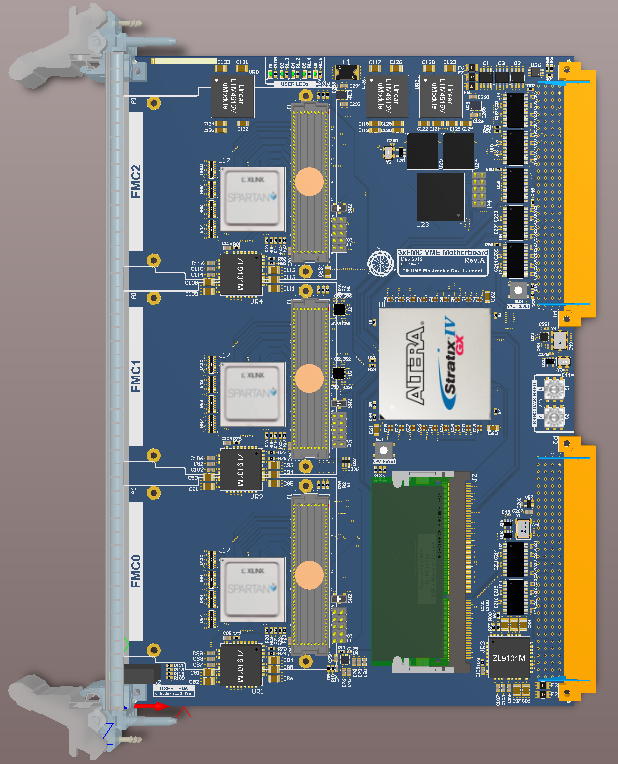
\includegraphics[height = 0.4\paperheight]{3xFMC_imageTOP}
\caption{The digitizer and trigger module motherboard. The three \gls{fmc} slots are labelled to the left of the board. Digital control is implemented on an Altera Stratix IV GX FPGA while interfacing with the \gls{fmc}s are controlled by the three Spartan-6 FPGAs.}
\label{Fig:DTM}
\end{figure}


%\begin{figure}[ht]
%\centering
%\includegraphics[height = 0.4\paperheight]{DTMModule}
%\caption{The digitizer and trigger module populated with the ADC, trigger I/O, and the clock mezzanine boards. Digital control is implemented on an Altera Stratix IV GX field programmable gate array.}
%\label{Fig:DTM}
%\end{figure}

\begin{figure}[ht]
\centering
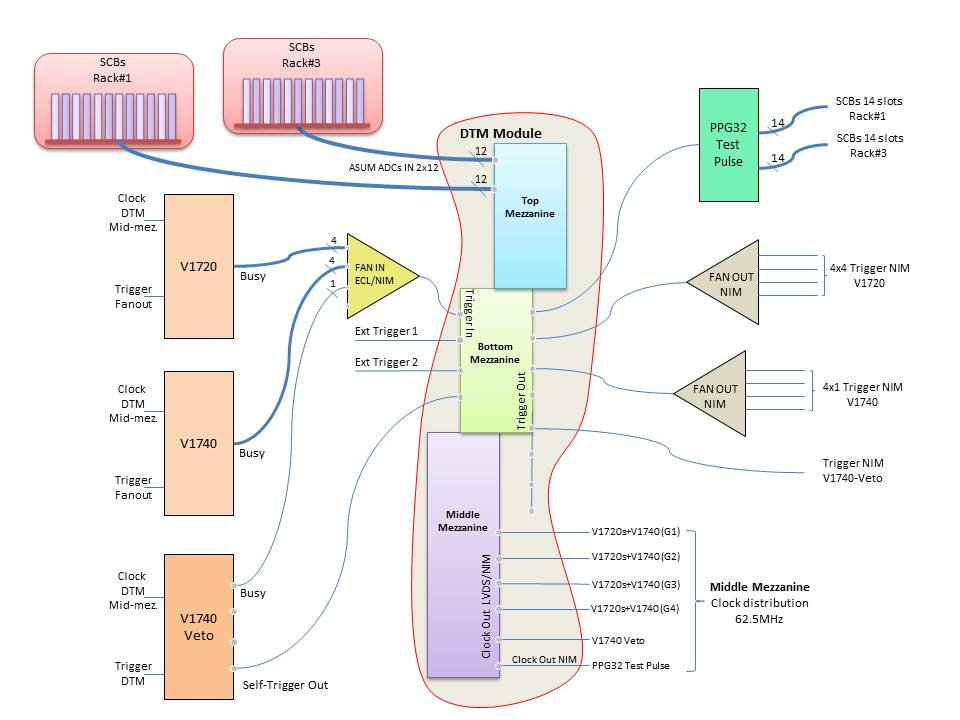
\includegraphics[width = 0.85\paperwidth]{daqSystemCartoon}
\caption{Diagram of the information and signal flow in the \gls{dtm}. The clock generator mezzanine board is shown as being used although this is subject to change (see Section \ref{sec:dtmConfigs} for more on the configurations)}
\label{Fig:daqSystemCartoon}
\end{figure}


\section{VME 3xFMC Carrier Motherboard}
\begin{description}
\item[EDEV Project Location: ]\url{https://edev.triumf.ca/svn/edevel00052}
\end{description}
Most modern experiments have many common characteristics when it comes to data acquisition, processing, and triggering. These mixed signal systems typically use some combination of fast ADC’s and general purpose I/O to capture and digitize any relevant data which is then piped into an \gls{fpga} for processing. Various data suppression algorithms and triggering schemes are implemented before the final events of interest are displayed or written to disk.
Large memory buffers are often necessary to prevent data loss and maximize the rate at which data can be acquired without overloading the processing capabilities of the \gls{fpga} or associated communication channels. The \gls{vme} 3x\gls{fmc} motherboard was conceived as a way to make better use of development resources. It was designed to meet these general needs while providing the flexibility to rapidly adapt to more specific project requirements.


An Altera Stratix IV GX \gls{fpga} (EP4SGX230KF40C2N)\footnote{\url{https://www.altera.com/products/fpga/stratix-series/stratix-iv/overview.html}} serves as the main processing and communication hub for the motherboard module. The \gls{vme} interface for the motherboard is provided by the Stratix IV GX \gls{fpga}. With the correct firmware, the motherboard fully supports all \gls{vme} data and addressing modes and may be implemented as most types of \gls{vme} module (Master, Slave, Arbiter, etc.). To support high speed ADCs and back-end communications (outside of \gls{vme}), this \gls{fpga} has 28 dedicated gigabit serial links going to the \gls{fmc} mezzanines (10, 10, and 8). Each link is capable of operating at data rates up to 8.5 Gbps.


Additional Xilinx Spartan-6 LX \gls{fpga}s (XC6SLX45-2FGG484I)\footnote{\url{http://www.xilinx.com/support/documentation/data_sheets/ds160.pdf}} are used for each of the three \gls{fmc}s providing support for bidirectional differential signalling (required by the \gls{fmc} specification).
The bidirectional differential signalling allows maximum compatibility for both custom and commercially available \gls{fmc} modules. 
Each \gls{fmc} interface on the carrier motherboard supports both single ended and differential I/O on banks LA and HA (except HA23), and single ended I/O and input only differential on bank HB (and HA23). 
This configuration gives a maximum per \gls{fmc} of 80 differential pairs (23 input only), 160 single ended I/O, or any combination thereof. 
Although the Spartan-6 LX \gls{fpga}s are mainly used for I/O interfacing, they also provide resources for additional data buffering, delay matching, and additional processing power. 

The carrier motherboard provides a very flexible clocking scheme. The \gls{vme} interface also provides a 16 MHz system clock.
On board oscillators provide fixed 16 MHz and 500 MHz clocks while a programmable oscillator (defaulting to 125 MHz) allows additional flexibility and a dedicated DDR3 memory interface reference clock. 
Each \gls{fmc} module may provide up to two dedicated gigabit transceiver reference clocks and two dedicated clock inputs which allow the option for mezzanine mounted oscillators or external clock inputs of any frequency.
All of these clock sources use dedicated \gls{pll} inputs on the Stratix IV GX and may be multiplied to any synthesizable frequency for driving internal logic or a wide variety of clock outputs.


To meet the data buffering and general computing memory requirements, the motherboard includes a 204 pin DDR3 SO-DIMM interface (laptop memory). 
The memory controller on the Stratix can supports up to 2 GB with a memory clock up to 533 MHz. 
This translates into a peak transfer rate of approximately 8.5 GB/s. For configuration management, an Altera MaxV CPLD (5M2210ZF256C5N)\footnote{\url{https://www.altera.com/content/dam/altera-www/global/en_US/pdfs/literature/hb/max-v/max5_handbook.pdf}} and 1Gb (2 x 512 Mb) of NOR flash memory is provided. The flash memory is directly accessible from the Stratix to allow for self programming and reconfiguration through \gls{vme} or other communication interfaces.
Uncompressed bitstreams for the Stratix IV GX and Spartan-6 \gls{fpga}s are 94,557,472 and 11,939,296 bits respectively so the provided flash allows support for several configurations for each with enough left over for some user data. 
While the CPLD handles the configuration of the Stratix, the configuration of the Spartan-6 \gls{fmc} interface \gls{fpga}s is managed by the main Stratix IV GX \gls{fpga}. This scheme allows for \gls{fmc} module identification and consequent reprogramming of the interface \gls{fpga}s.


Power management on the motherboard has also been implemented to allow maximum flexibility. The power design supports use in \gls{vme} crates with or without the 3.3V supply provisioned in the VME64X spec\footnote{For the standard see: \url{http://file.wiener-d.com/documentation/General/WIENER_VME_VXI_VXS_introduction_1.0.pdf}}. 
While all supply voltages are provided regardless of the crate used, additional power is available for the individual \gls{fmc} modules when the 3.3V supply is present. 
Each \gls{fmc} slot is supplied with a 12V ($<$1A) and 3.3V ($<$3A) fixed supplies and a dedicated 0-3.3V adjustable supply, VADJ ($<$4A). 
In return, the \gls{fmc} modules provide the carrier with I/O voltage for bank B and reference voltage for banks A and B if voltage referenced I/O standards are used.
All of the power supplies are monitored and controlled from the Stratix IV GX \gls{fpga} on the carrier motherboard.


The \gls{vme} 3x\gls{fmc} Carrier Motherboard is a very flexible and capable card, however, most of the actual functionality comes from the \gls{fmc} modules that are physically plugged in whether custom built or commercially available.



\subsection{Motherboard Components}
The major components of the \gls{dtm} consist of the following:

\begin{description}
	\item[(1) Altera Max V CPLD] \hfill \\
	On power-up configures the Stratix IV FPGA, and allows JTAG programming of both the Stratix IV and the Flash memory. Also performs watchdog on Stratix IV.
	
	\item[(1) Altera Stratix IV FPGA] \hfill \\
	Core of the \gls{dtm}. Performs \gls{vme} transfers, runs NIOSII embedded processors, trigger system, and configures the Spartan-6s. Only \gls{fpga} with direct access to DDR3 SDRAM, LEDs, switches, and \gls{vme}. Shares bus to Flash memory with Max V.
	
	\item[(1) DDR3 SDRAM DIMM] \hfill \\
	Used for ADC data storage
	
	\item[(2) 512 Mb Flash Memory Chips] \hfill \\ 
	Contain configuration files for Stratix IV and Spartan-6 FPGAs. 
	
	\item[(3) Xilinx Spartan-6 LX FPGAs] \hfill \\
	Used to decode ADC, initialize the clock module, and connect the FMCs I/O to the Stratix IV.
	
	\item[(3) FMC connectors] \hfill \\ 
	Where the mezzanine cards go.
	
	\item[(9) User-controlled LEDs] \hfill \\ 
	Diagnostics and status
	
	\item[(2) User-controlled 16 position switches] \hfill \\ 
	Set VME address of DTM
	
	\item[(1) VME64 compatible backplane] \hfill \\ 
	Communication link of DTM
\end{description}


\subsection{Board Revisions}

There have been two revisions of this motherboard to date, Rev.A and Rev.B\footnote{See the errata for firmware compatibility issues (Chapter \ref{chap:errata})}. The primary difference between these revisions is only the addition of a SD card on Rev.B. Although the hardware is essentially identical there were issues that arose which meant that the firmware release edevel00268 only worked on Rev.B boards although this issue has been fixed in the newer edevel00365 releases and the boards can now be used interchangeably (See Chapter \ref{chap:firmware} and \ref{chap:errata}).

\subsection{Board Settings $\&$ Registers}
\subsubsection{VME Address}
\begin{description}
\item[Twiki Location: ]\url{https://www.snolab.ca/deap/private/TWiki/bin/view/Main/Dtmboard}
\end{description}
The motherboard is equipped with two rotary switches for setting the \gls{vme} base address. Default setting is 0x69 = sw2[7-4]: 0110, sw1[3-0]: 1001. \textbf{Bit 0}, the boot bit, \textbf{must always be on}. Bit[7-4][3-0] $\rightarrow$ 0110 1001 $\rightarrow$ 0xB(3,7-5) corresponding to the upper 4 bits of the A24: 0xB00000 (Rotary switch: 0x69), bit[7-4][3-0] $\rightarrow$ 1000 1001 $\rightarrow$ 0xC(3,7..5) corresponding to the upper 4 bits of the A24: 0xC00000 (Rotary switch: 0xC9).

The \gls{vme} base address has to be adjusted correspondingly in the frontend or access code (deap/pro/FrontEnd/dtm/vme\_register.h (DTM\_BASE)). No two \gls{vme} modules being used can use the same base address. %\footnote{See the errata for base address changes (Section \ref{sec:baseAddressErrata})}. 

\subsubsection{DTM Registers}
\begin{description}
\item[Twiki Location: ]\url{https://www.snolab.ca/deap/private/TWiki/bin/view/Main/Dtmregisters}
\end{description}

In general, there exist two type of registers: ReadWrite (RW) and ReadOnly (RO). The first type is used to set parameters through \gls{odb} (see Section \ref{sec:odb}), the second one to read the status and data of the different \gls{dtm} firmware modules. The last two bits of the address are not used, therefore the distance between registers is 0x4 in address space.

The exact register address is given by:

DTM\_BASE + (RW/RO/USER)\_OFFSET + REG\_OFFSET

Reading of these registers can be done over \gls{jalisco} (see Section \ref{sec:jalisco}) or using \gls{vme} command line commands using vme\_read.exe -b 0xb00000 (which is the dtm base) -a (register address)\footnote{See the twiki for how to run this:\\ \url{https://www.snolab.ca/deap/private/TWiki/bin/view/Main/UsingTriumfDtmTestSetup}}.

\NOTE{The registers in \gls{jalisco} are displayed in 32 bit words, so the \gls{jalisco} offset is the register table offset/4.}

\section{Mezzanine Boards $\&$ DTM Connections}
The following describes the different \gls{fmc} boards used and connections in the various \gls{dtm} configurations. The different configurations themselves are discussed in Section \ref{sec:dtmConfigs} with their associated firmware in Chapter \ref{chap:firmware}.

\subsection{24 Channel ADC FMC}
\label{sec:adcBoard}
\begin{description}
\item[SVN Project Location: ]\url{https://edev.triumf.ca/svn/edevel00018}
\item[SVN Firmware Location: ]\url{https://edev.triumf.ca/svn/edevel00230}
\item[Hardware Connections: ]\url{https://www.snolab.ca/deap/private/TWiki/bin/view/Main/HWconnection#FMCADC}
\end{description}
The ADC (or Digitizer) board, seen in Fig. \ref{Fig:adcBoard} is populated with three eight channel 12-bit 45 \gls{msps} $\Sigma - \Delta$ ADCs (ADC12EU050)\footnote{Data sheet: \url{http://www.ti.com/lit/ds/symlink/adc12eu050.pdf}}. 
The \gls{dtm} receives 22 analog sums (\gls{asum}s) of 12 \gls{pmt} signals from the \gls{scb}s which are digitized by the ADC mezzanine board\footnote{Have a look at the \gls{deap3} technical manual or the \gls{deap} electronics paper}. These digitized \gls{asum}s are used to make the trigger decision as discussed in Chapter \ref{chap:triggers}. 

The \gls{scb} \gls{asum} output signals are received on differential lines by the ADC. The differential common mode is 0.6 V.
To match the ADC $\pm$1.05 V dynamic range the \gls{scb} applies a constant offset of 0.8 V to the \gls{asum} signal.
The ADC are supplied a 45.161290 MHz clock by a \gls{pll} on the \gls{dtm}\footnote{Other documentation reports a 50 MHz clock to the ADCs, that is out of date. This is the maximum allowed speed of the ADCs.}.

\NOTE{The PLL is set to 45.25 MHz but the 45.161290 MHz is the fastest it can run, hence the odd rate.}

To ensure a low jitter clock for sampling and data transfer off the ADC, this clock is first passed through a clean-up \gls{pll} integrated into the ADC. 
The 12-bit data sampled by the ADC at 45.161290 MHz is transferred to the Spartan-6 \gls{fpga} as serial DDR data.% at 350 MHz along with a corresponding 350 MHz bit clock \FIXME{IS THIS RATE CORRECT?}.
To enable the correct re-alignment of the 12-bit data word in the \gls{fpga} a word clock is also provided by the ADC. Control of the ADC is performed via a serial to parallel interface (SPI) command protocol.
To test data alignment the ADC provides default test patterns and a user defined test pattern. The test patterns are enabled and in the case of the user test pattern defined over the SPI command structure.
\gls{jalisco} includes tools for reading and debugging ADC's, refer to Section \ref{sec:jalisco}.

\textbf{Configuration Notes:} Unchanged board used in all configurations of the \gls{dtm} and for firmware modules edevel00268 and edevel00365.

\begin{figure}
\centering
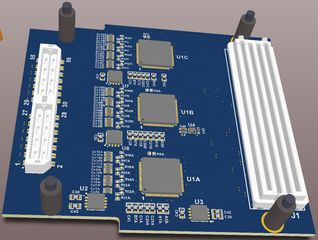
\includegraphics[width = .5\textwidth]{adcBoard}
\caption{24 Channel digitizer board which receives 22 analog sums of 12 \gls{pmt}s each and passes the digitized result to the main Stratix IV \gls{fpga} for a trigger decision to be made.}
\label{Fig:adcBoard}
\end{figure}


\subsection{DEAP Clock Generator Module}
\label{sec:mClockBoard}
\begin{description}
\item[SVN Project Location: ]\url{https://edev.triumf.ca/svn/edevel00114}

\item[SVN Firmware Location: ]\url{https://edev.triumf.ca/svn/edevel00230}

\item[Hardware Connections: ]\url{https://www.snolab.ca/deap/private/TWiki/bin/view/Main/HWconnection#FMCCLOCK}
\end{description}

The clock generator board distributes an 62.5 MHz clock generated in the Stratix IV to the rest of the \gls{daq} system via a daisy chain arrangement. These are distributed as: four clock signals to the four \gls{v1720} sectors; one clock signal to the \gls{v1740} sector; and one clock signal to the \gls{ppg} module. The 62.5 MHz clock distribution to the four \gls{v1720} sectors, the \gls{v1740} sector and the \gls{ppg} as discussed in Section \ref{sec:daisyChainClock}.
Within the \gls{v1720} and \gls{v1740} sectors the clock signal is daisy chained module to module (see Section \ref{sec:newClock}).

The clock generator \gls{fmc} has seven \gls{lvds} and three \gls{nim} I/O ports. Five \gls{lvds} are used to connect to each of the four clock groups and the VETO \gls{v1740}s. One \gls{nim} port is used for the \gls{ppg} clock. The remaining ports are unassigned general I/O\footnote{See \url{https://www.snolab.ca/deap/private/TWiki/bin/view/Main/HWconnection}}.

\textbf{Configuration Notes:} Board used in all releases of firmware module edevel00268, replaced with the SFP and Mini-SAS board in mezzanine (See Section \ref{sec:SFPBoard}). Last stable release installed at SNOLAB using this board edevel00268/\tagTwoSixEight. See Section \ref{sec:dtmConfigs} for the different \gls{dtm} configurations, and Section \ref{sec:newClock} for more on the \gls{dtm} and \gls{daq} clocking system.

\begin{figure}
\centering
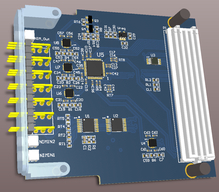
\includegraphics[width = .5\textwidth]{mClockBoard}
\caption{Seven \gls{lvds} and three \gls{nim} I/O ports configured to provide the master clock to the rest of the \gls{daq} system in a daisy chain clocking configuration (see Section \ref{sec:daisyChainClock}).}
\label{Fig:mClockBoard}
\end{figure}



\subsection{SFP and Mini-SAS Interface}
\label{sec:SFPBoard}
\begin{description}
\item[SVN Project Location: ]\url{https://edev.triumf.ca/svn/edevel00228}
\item[SVN Firmware Location: ]\url{https://edev.triumf.ca/svn/edevel00230}
\end{description}
\noindent This module is equipped with:
	\begin{enumerate}
	\item (1) SFP connector allowing gigabit ethernet
	\item (1) Mini-SAS connector
	\item (1) eSATA connector (can be configured as a clock in)
	\item (1) Micro-SD card
	\end{enumerate}

The SFP and Mini-SAS Interface \gls{fmc} has been designed for the \gls{deap3} experiment to add ethernet networking and data storage on the on-board micro-SD card, see Chapter \ref{chap:install} for interfacing and features.

\begin{figure}
\centering
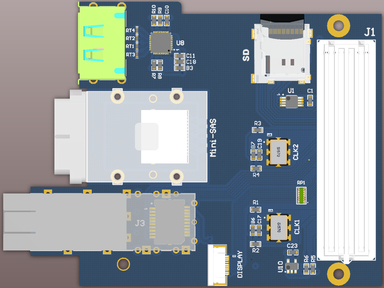
\includegraphics[width = .5\textwidth]{ethernetBoard}
\caption{SFP ethernet and Mini-SAS interface board which adds FTP readout and flash programming interfacing with the \gls{dtm} (see Chapter \ref{chap:install})}
\label{Fig:ethernetBoard}
\end{figure}


\subsection{DEAP NIM I/O Trigger Module}
\label{sec:nimBoard}
\begin{description}
\item[SVN Project Location: ]\url{https://edev.triumf.ca/svn/edevel00019}
\item[SVN Firmware Location: ]\url{https://edev.triumf.ca/svn/edevel00279}
\item[Hardware Connections: ]\url{https://www.snolab.ca/deap/private/TWiki/bin/view/Main/HWconnection#FMCIO}
\end{description}
The \gls{nim} I/O board is a twelve channel \gls{nim} board used for trigger output, \gls{daq} control/status, calibration systems control, and in one configuration a master clock output\footnote{See the configuration notes and Section \ref{sec:dtmConfigs}}. 

The twelve channels are split between eight dedicated outputs and four dedicated inputs.
The \gls{v1720} and \gls{v1740} can both accept \gls{nim} or TTL logic \cite{v1720UM}\cite{v1740UM}, for compatibility with the \gls{ppg}\cite{ppg} \gls{nim} logic is chosen.
The \gls{v1720} and \gls{v1740} boards specify \gls{nim} lemo-00 50$\Omega$ trigger input connections, the \gls{ppg}\cite{ppg} specifies \gls{nim} lemo-00 inputs.
Due to space limitations the I/O board is populated with mmcx connectors\footnote{These are fragile and very prone to breaking}.

\begin{figure}
\centering
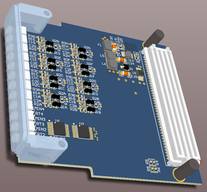
\includegraphics[width = .5\textwidth]{nimBoard.jpg}
\caption{12 Channel \gls{nim} I/O board used for controlling the rest of the \gls{daq} system including the output of the trigger signal and busy inputs. In one \gls{dtm} configuration this board also outputs the master clock (see Section \ref{sec:dtmConfigs}).}
\label{Fig:nimBoard}
\end{figure}

\subsubsection{Trigger Distribution}
On the generation of a trigger signal by the \gls{dtm}, or an external trigger input, a trigger signal is distributed to the \gls{daq} system through the \gls{nim} board. 
The trigger signal is distributed on five dedicated trigger lines to the \gls{v1720} and \gls{v1740} sectors.
For the purposes of clock and trigger distribution, the \gls{v1720} and \gls{v1740} digitizers are grouped into five logical sectors (Fig. \ref{Fig:triggerDist}). 
The 32 \gls{v1720}s are grouped into four sectors where each logical sector contains eight physical modules. 
The \gls{v1740} modules form a single logical trigger and clock sector. 
Each logical trigger sector receives a single trigger signal distributed from the \gls{nim} board. 
The signal is received by the first board in each sector and then daisy chained, board to board, within each sector.


\begin{figure}
\centering
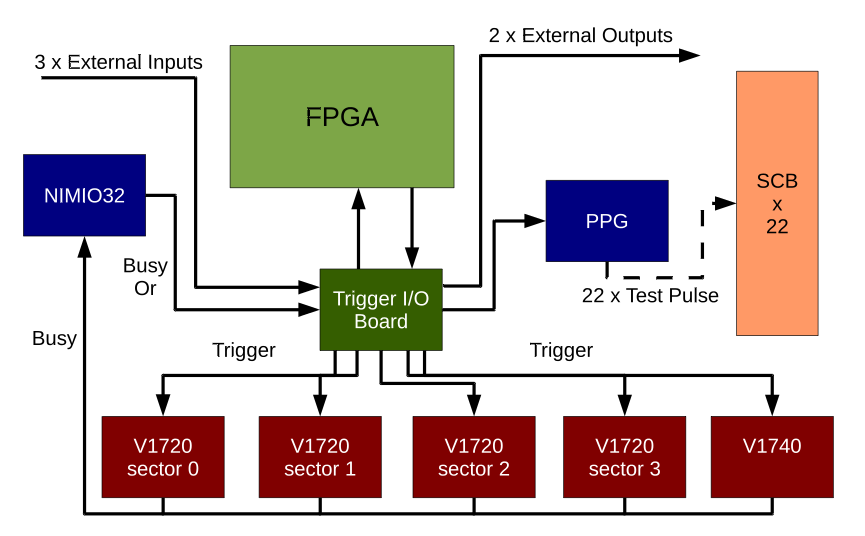
\includegraphics[width = \textwidth]{triggerDist}
\caption{Diagram of the trigger signal distribution in the \gls{daq} system.}
\label{Fig:triggerDist}
\end{figure}

\NOTE{For more on the busy signals, see the \href{https://www.snolab.ca/deap/private/TWiki/bin/view/Main/BusySystem}{Twiki}\footnote{\url{https://www.snolab.ca/deap/private/TWiki/bin/view/Main/BusySystem}}}

\section{Clocking} 
\label{sec:newClock}

Currently\footnote{Using edevel00268 July, 2016} the clock distribution and thereby the synchronization of events for the \gls{dtm} and the \gls{v1720} and \gls{v1740} digitizers is done through a daisy chain arrangement.

The stability of this arrangement has been brought into question as some trigger signals were found to be arriving close to the clock boundary. This is an issue as the \gls{v1720} clock delays are only allowed to be certain values rather than arbitrary precision so the tuning of delays is limited. The issue has not arisen after the clock delays were readjusted. Further issues with the daisy chain clocking is that the cables are flaky. 
To address these potential problems a new clock distribution system has been developed. 
The daisy chained \gls{dtm} generated master clock is to be replaced with a \gls{vme} clock distribution system with the master clock being sourced from the \gls{dtm} via the unused output on the NIM I/O board. The clock distribution modules\footnote{\url{https://edev.triumf.ca/project/edev/vme/edevel00163}}, replace the need for a daisy chain arrangement and thereby removing a potential source of error. The clock generator \gls{fmc} on the \gls{dtm} is to be replaced with a SFP and Mini-SAS \gls{fmc}.

\subsection{Daisy Chain Clocking}
\label{sec:daisyChainClock}
The master clock for the \gls{daq} system is generated from the motherboards 50 MHz source clock. A phase lock loop (\gls{pll}) on the \gls{dtm} sets the frequency to 100 kHz for the periodic trigger (see Section \ref{sec:periodicTrigger}), and 62.5 MHz clock for the \gls{ppg} module and the digitizers. The dedicated clock generator mezzanine board passes the 62.5 MHz clock to the first digitizer in groups of at most six which is then passed along the chain. To match the expected trigger delay introduced by daisy chaining, a 3.57 ns delay is added to the clock daisy chain. The clock delay is configurable within the \gls{v1720} or \gls{v1740} modules as described by the manufacturer\cite{v1720UM}\cite{v1740UM}. 

\begin{figure}
\centering
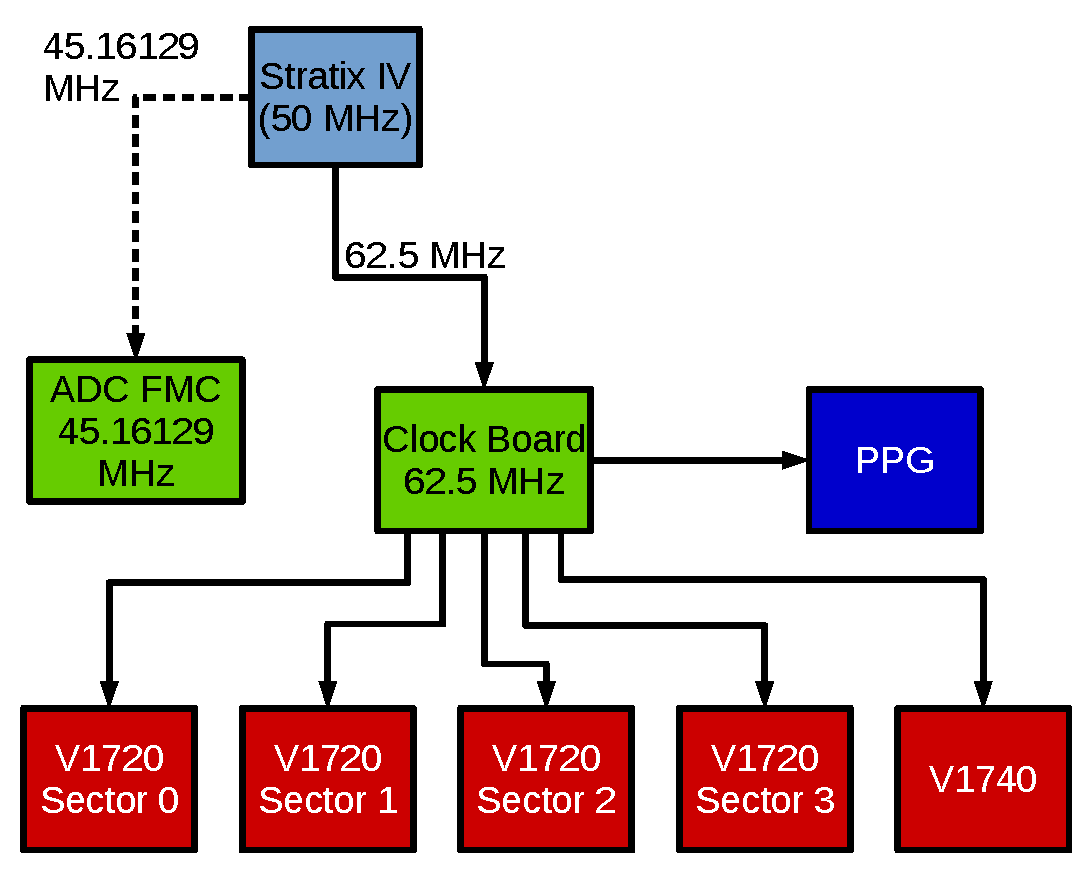
\includegraphics[height = 0.36\paperheight]{daisyChain}
\caption{Clocking diagram of the data acquisition system under the daisy chain configuration}
\label{Fig:daisyChainClock}
\end{figure}

\subsubsection{Distributed Master Clock}
\label{sec:distributedMasterClock}

Replacing the daisy chain clocking is a distributed system removing the necessity of setting delays in the chain. The distributed system used the Clock Distribution Modules\footnote{\url{https://edev.triumf.ca/project/edev/vme/edevel00163}} (\gls{cdm}) designed by the TRIUMF EDEV department for use on the GRIFFIN project. The 62.5 MHz \gls{daq} master clock is generated in the \gls{dtm} and fed through the NIM I/O \gls{fmc} to the first of three the \gls{cdm}. This first slave \gls{cdm} cleans the clock and outputs two synced, phase locked clocks to two other \gls{cdm}s which then fan out all of the \gls{daq} clocks. As the same wire is used for all connections and the sources are synced and phase locked, there is no need for any programmed delays. 


\begin{figure}
\centering
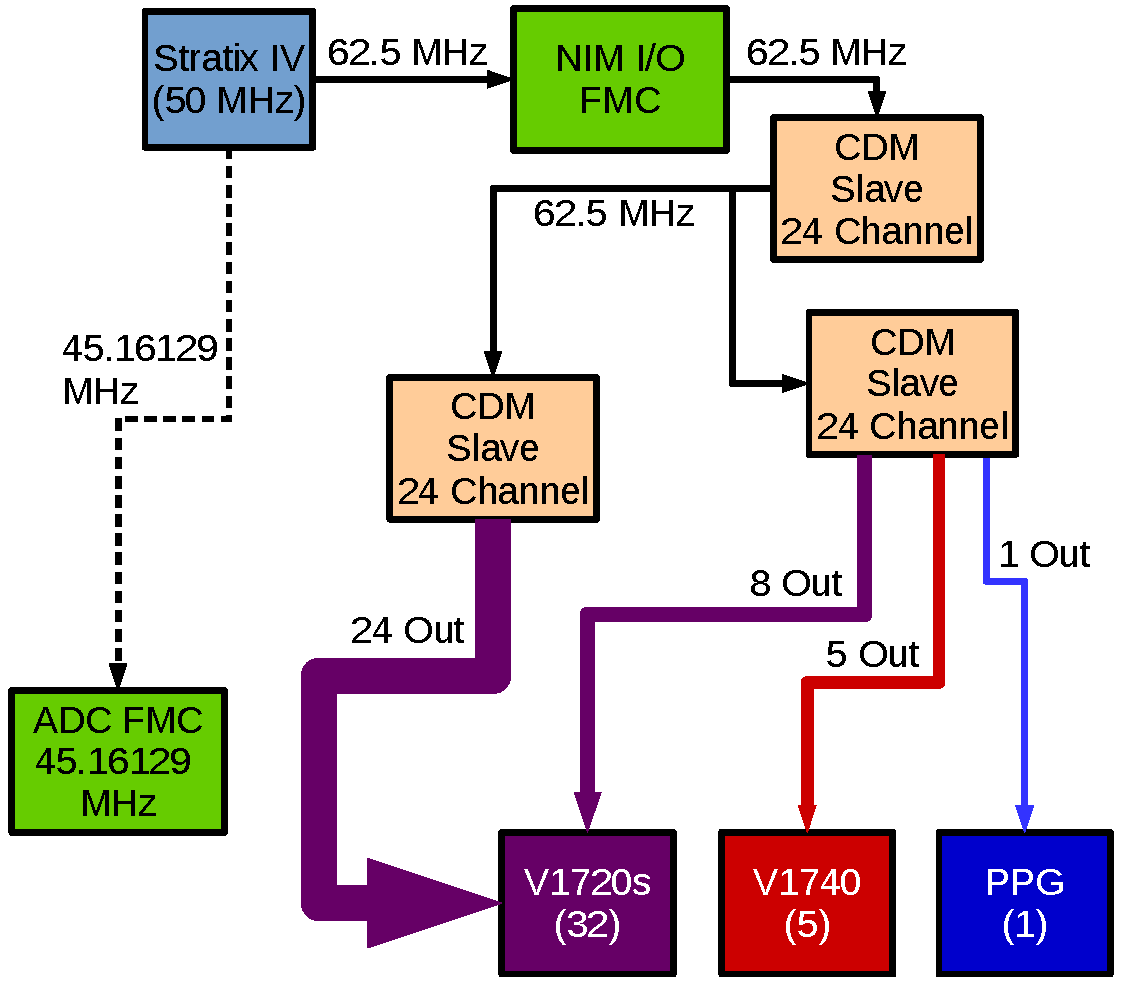
\includegraphics[height = 0.36\paperheight]{distClock}
\caption{Diagram of the clock distribution system for the data acquisition system using a distributed master clock method, replacing the daisy chain configuration in Fig. \ref{Fig:daisyChainClock}.}
\label{Fig:distClock}
\end{figure}
\clearpage
\subsubsection{Clock Distribution Modules}
\begin{description}
\item[EDEV Project Location:] https://edev.triumf.ca/project/edev/vme/edevel00163
\item[Summary:] 24 channel low jitter \gls{lvds} Clock/Sync generation and fan out module
\end{description}
The clock distribution modules, shown in Fig. \ref{Fig:clockDistMod}, are the essential part of the clock distribution system. Designed for the GRIFFIN experiment by the TRIUMF EDEV department, these boards output a stable and phase locked clock through up to 24 channels. 
\begin{figure}
\centering
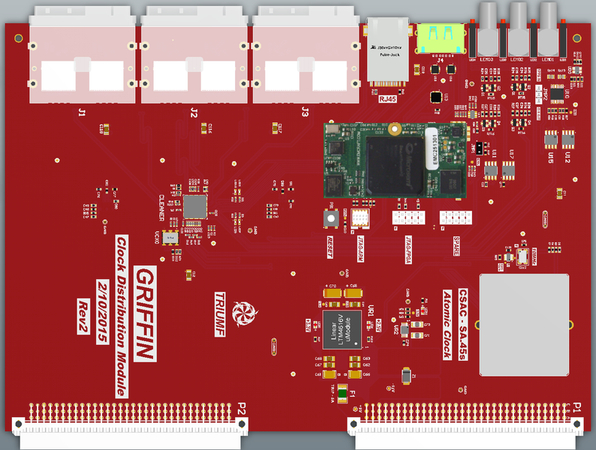
\includegraphics[height = 0.36\paperheight]{clockDistMod}
\caption{Clock distribution module to be used for the distributed clocking of the system, supplanting the current (July 2016) \gls{daq} daisy chain method.}
\label{Fig:clockDistMod}
\end{figure}

\section{DTM Configurations}
\label{sec:dtmConfigs}
There are two \gls{fmc} configurations used for the \gls{dtm}, both use the same NIM I/O and 24-channel ADC \gls{fmc}s but switch out the clock generator (Fig. \ref{Fig:dtmConfig268}) with the SFP and Mini-SAS board (Fig. \ref{Fig:dtmConfig365}). This change of boards is due to an intended\footnote{Not yet installed at SNOLAB as of July 2016} change in the clock distribution method from a daisy-chain to a distributed phase-locked clock system (see Section \ref{sec:newClock}). The addition of the SFP connection comes with added ethernet capabilities allowing ethernet data readout to replace the current VME readout system (see Chapter \ref{chap:install} for more on the FTP and ethernet data readout). The firmware project that uses the clock generator module is edevel00268 (Section \ref{sec:268}) and the SFP and Mini-SAS project is edevel00365 (Section \ref{sec:365}).
\begin{figure}
\centering
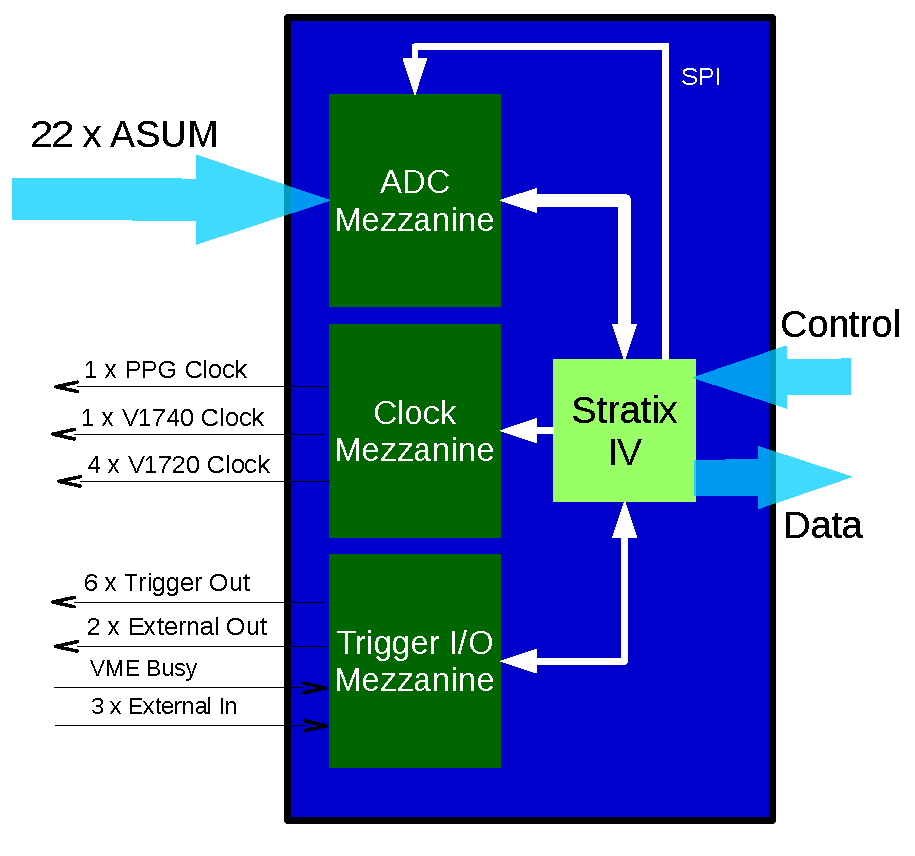
\includegraphics[height = 0.36\paperheight]{dtmConfigClockBoard}
\caption{DTM configuration using the edevel00268 firmware project (see Section \ref{sec:268}). The master clock is generated by the Stratix IV and fed out to the digitizers and externals through the clock generator module (Section \ref{sec:daisyChainClock}). The master clock is fed out to first in a section of digitizers and is passed along in a daisy chain with delays programmed into the digitizers as described in section \ref{sec:daisyChainClock}.}
\label{Fig:dtmConfig268}
\end{figure}

\begin{figure}
\centering
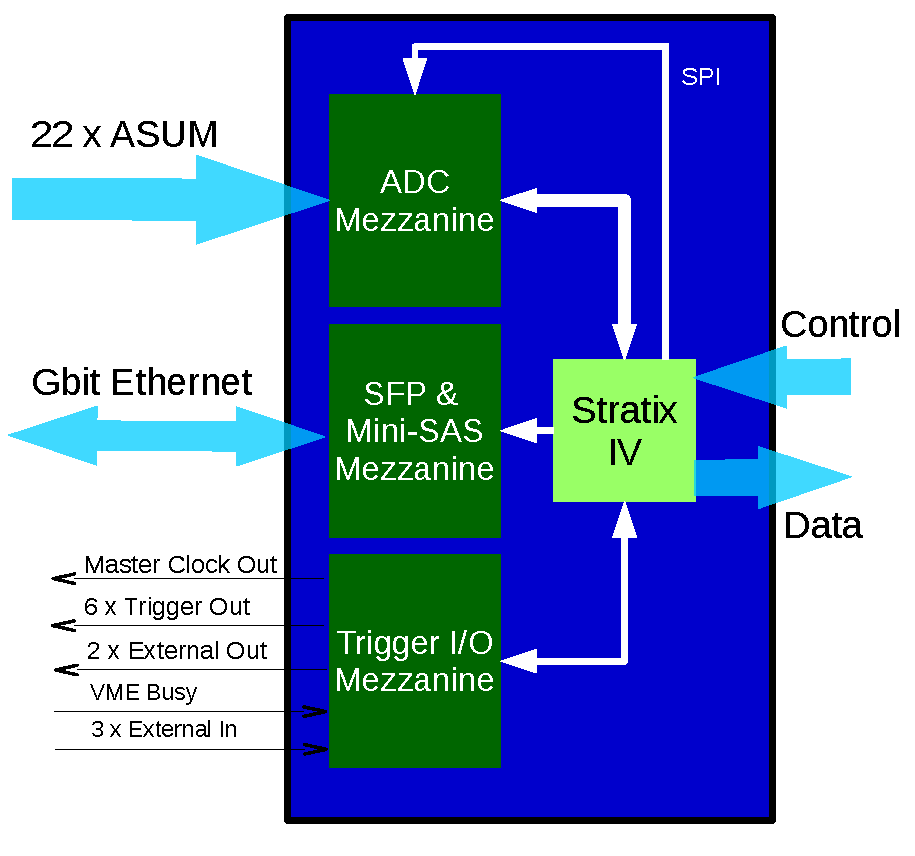
\includegraphics[height = 0.36\paperheight]{dtmConfigSFPMasterClockOut}
\caption{DTM configuration using the edevel00365 firmware project (see Section \ref{sec:365}). The master clock is generated by the Stratix IV and fed out to the digitizers and externals through the NIM I/O module. The master clock is then sent to a clock distribution module in slave mode which feeds out two cleaned, phase locked, and synchronized clocks to two more clock distribution modules in slave mode (see Section \ref{sec:distributedMasterClock}). A SFP and Mini-SAS \gls{fmc} replaces the clock generator board which adds FTP connectivity and ethernet readout of the registers.}
\label{Fig:dtmConfig365}
\end{figure}

\chapter{Trigger Types}
\label{chap:triggers}

There are five primary trigger types currently implemented in the \gls{deap3} firmware: periodic, exponential, external, minimum bias, and the ADC trigger. The trigger types, operation, and user settings are discussed below. More on the \gls{odb} can be found in Section \ref{sec:odb} with the settings and variable descriptions in the \href{https://www.snolab.ca/deap/private/TWiki/bin/view/Main/Dtmodb}{twiki}. This chapter borrows from the \href{https://www.snolab.ca/deap/private/TWiki/bin/view/Main/Triggerproject}{twiki, the link to which can be found here}.

\NOTE{Simulation information can be found on the \hypNote{twiki}{https://www.snolab.ca/deap/private/TWiki/bin/view/Main/FirmwareSimulation}}
\section{Periodic}
\label{sec:periodicTrigger}

\begin{description}
\item[SVN Location: ]https://edev.triumf.ca/svn/edevel00261/trunk/tsb/ip/rtl/source/ts\_periodic.v
\item[Module Name: ]TriggerSourcePeriodic
\item[Frequency Range: ]1 Hz $\rightarrow$ 100 kHz
\item[Submodules: ]None
\item[Summary: ]Used for testing the \gls{daq} system with a periodic signal (fixed interval between triggers). Uses a 100 kHz \gls{pll} and a counter to divide the rate. This trigger does not have a separate module, but is included in the \gls{vme} wrapper in edevel00270\footnotemark[\value{footnote}]. The periodic trigger has two identical channels used for the \gls{ppg} pulse injection, \gls{aarf} firing, status updates, etc.
\end{description}

\begin{landscape}
	\vspace*{\fill}
	\begin{figure}[ht]
	\centering
	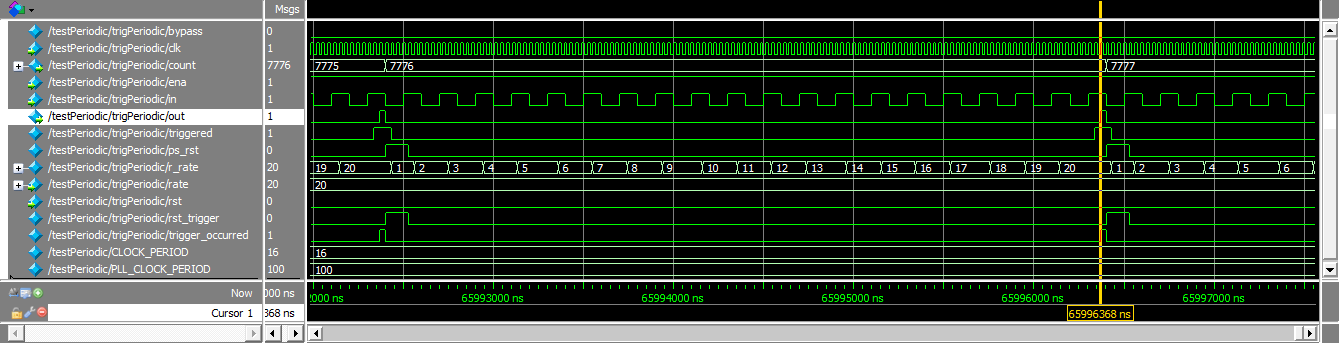
\includegraphics[width = \paperwidth]{periodicSim.png}
	\caption{Timing diagram for the periodic trigger.}
	\label{Fig:periodicTime}
	\end{figure}
	\vspace*{\fill}
\end{landscape}

\subsection{ODB Settings}
\label{sec:periodicODB}

\begin{figure}[ht]
\centering
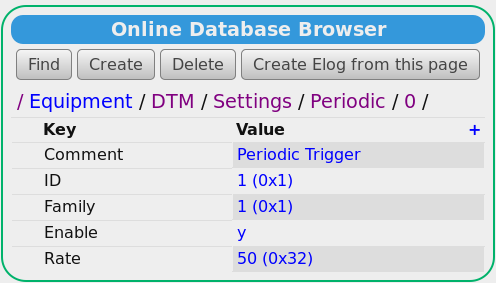
\includegraphics[width = 0.5\paperwidth]{periodicODB}
\caption{Online data base settings for the periodic trigger.}
label{Fig:periodicODB}
\end{figure}

\begin{description}
\item \textbf{Trigger ID: } Two identical channels
	\begin{description}
	\item \textbf{Channel 0: }0x1
	\item \textbf{Channel 1: }0xFFFFFFFF
	\end{description}

\item \textbf{Family: } 0x1 (Periodic)

\item \textbf{Enable: }Turns the trigger module on/off

\item \textbf{Rate: }Set rate of the trigger in Hz (1 $\rightarrow$ 10$^5$ Hz)
\end{description}

\section{Exponential}


\begin{description}
\item[SVN Location: ]https://edev.triumf.ca/svn/edevel00261/trunk/tsb/ip/rtl/source/ts\_exponential.v
\item[Module Name: ]TriggerSourceExponential
\item[Frequency Range: ]1 Hz $\rightarrow$ 62.5 MHz
\item[Submodules: ]None
\item[Summary: ] Used for testing the \gls{daq} system with exponentially distributed random intervals between triggers. Can emulate LAr background decay trigger rate, PMT dark noise trigger rate, expected event trigger rate $\rightarrow$ Emulates real \gls{daq} conditions. Uses a C++ program running on a NIOS core that generates the exponentially distributed random numbers for all 5 trigger sources, a FIFO to store those numbers and a counter that generates the trigger when the next random number is reached. The rate is more correctly the mean of the distribution from which delay times are taken, so the rate here is actually the time averaged rate.
\end{description}

\subsection{ODB Settings}
\label{sec:expODB}
\begin{figure}[ht]
\centering
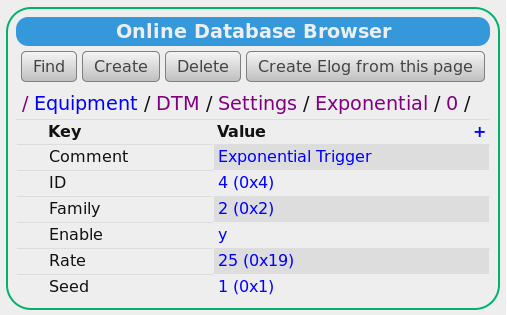
\includegraphics[width = 0.5\paperwidth]{expODB}
\caption{Online data base settings for the exponential trigger.}
\label{Fig:expODB}
\end{figure}
 

\begin{description}
\item \textbf{Trigger ID: } Five different identical channels
	\begin{description}
	\item \textbf{Channel 0: }0x4
	\item \textbf{Channel 1: }0x8
	\item \textbf{Channel 2: }0x10
	\item \textbf{Channel 3: }0x20 
	\item \textbf{Channel 4: }0x40 
	\end{description}

\item \textbf{Family: } 0x2 (Exponential)

\item \textbf{Enable: }Turns the trigger module on/off

\item \textbf{Rate: }Average rate of the trigger in Hz

\item \textbf{Seed: }Seed value for the random number generator
\end{description}
 
\section{External}
\begin{description}
\item[SVN Location:] https://edev.triumf.ca/svn/edevel00261/trunk/tsb/ip/rtl/source/ts\_external.v
\item[Module Name: ]TriggerSourceExternal
\item[Frequency Range: ] 0 Hz $\rightarrow$ 62.5 MHz (Pulses must be at least 16 ns wide)
\item[Submodules: ]None
\item[Summary: ]External triggers are sourced from the veto PMTs and the calibration devices via the \gls{nim} I/O \gls{fmc} (Section \ref{sec:nimBoard}). These external triggers are primarily intended for the removal of muon events which can be tagged by the veto system as they create Cerenkov radiation in the water tank. There are three identical channels, one for the veto system and two of which are currently unassigned\footnote{July 2016}.
\end{description}
\begin{landscape}
	\vspace*{\fill}
	\begin{figure}[ht]
	\centering
	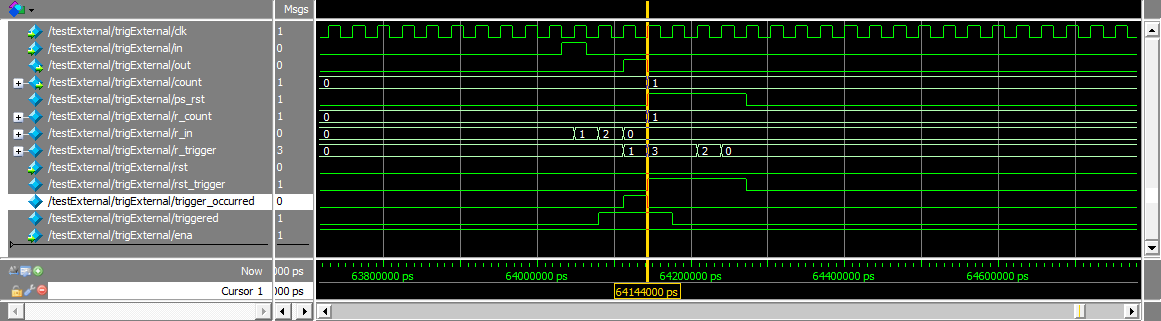
\includegraphics[width = \paperwidth]{externalSim.png}
	\caption{Timing diagram for the external trigger.}
	\label{Fig:}
	\end{figure}
	\vspace*{\fill}
\end{landscape}

\subsection{ODB Settings}
\label{sec:externalODB}

\begin{figure}[ht]
	\centering
	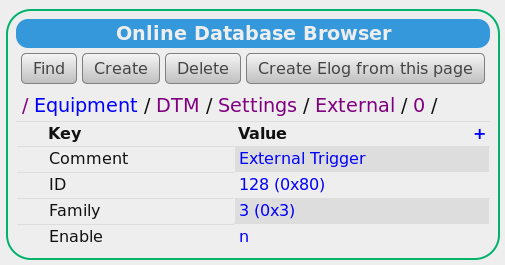
\includegraphics[width = 0.5\paperwidth]{externalODB}
	\caption{Online data base settings for the external trigger.}
	\label{Fig:externalODB}
\end{figure}


\begin{table}
	\centering
	\caption{Trigger ID and connections for the external trigger}
	\begin{tabular}{l l l l}
	Channel&	Trigger ID&		NIM Channel&	Application\\ \hline \hline	
			0&		0x80&				0&				Veto\\  
			1&		0x100&				1&				Calib\\ 
			2&		0x200&				2&				External Trigger 2\\ \hline \hline		
	\end{tabular}
\end{table}

\begin{description}
\item \textbf{Family: } 0x3 (External)

\item \textbf{Enable: }Turns the trigger module on/off
\end{description}

\section{Minimum Bias}
\label{sec:minBias}
\begin{description}
\item[SVN Location:] https://edev.triumf.ca/svn/edevel00261/trunk/tsb/ip/rtl/source/ts\_adc\_min\_bias.v
\item[Module Name: ]TriggerSourceADCMinimumBias
\item[Frequency Range: ]Settings Dependant, minimum time between triggering four clock delay (Reset and flip-flop setting) + dead time + \gls{tot} time (see Fig. \ref{Fig:minBiasSingleSim} and \ref{Fig:minBiasCoincSim})
\item[Submodules: ]min\_bias\_sum (channel counting megafunction)
\item[Summary: ]The minimum bias trigger compares the \gls{asum} data to a threshold set in the online data base \gls{odb}. If the signal stays above this threshold for a certain defined time known as the time over threshold (\gls{tot}), then the channel is said to have latched (diagram in Fig. \ref{Fig:minBiasTrigger}). The \gls{tot} requirement is intended to reduces the chance of triggering on noise.

There are two modes for the min. bias trigger: single channel or coincidence mode. In single channel mode, once one channel latches the trigger condition is met and a trigger signal is sent. In coincidence mode multiple channels need to latch within a definable amount of time known as the coincidence time window. In coincidence mode once the last channel has latched a trigger signal is sent. 

Once a trigger condition has been met and a trigger signal output, the trigger goes into a dead state until the defined deadtime has been passed. The deadtime is intended to reduce the chance of retriggering on the same event.
 
 \NOTE{The minimum bias can be used with the 22 \gls{asum} channels and the \gls{ass}, which channels are enabled are set in the \gls{odb}.}
 %In order to readout the \gls{dtm} ADC waveform data corresponding to the trigger, an ADC FREEZE FIFO LATENCY of about 2500 cycles (62.5 MHz) is required with the current FIFO settings. 
\end{description}

\begin{figure}[ht]
\centering
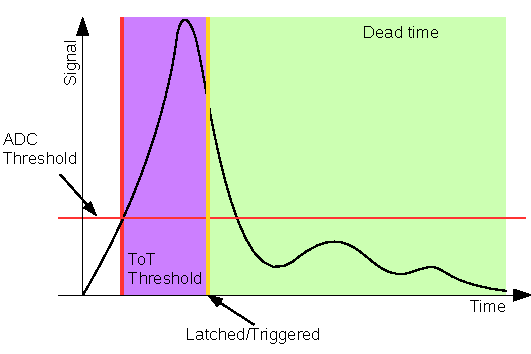
\includegraphics[width = 0.7\paperwidth]{minBiasTrigger.pdf}
\caption{Cartoon depicting the operation of the minimum bias trigger. The trigger fires once the signal has remained above the adc threshold (horizontal line) for the time over threshold (vertical red line) at which point the trigger will fire immediately (vertical yellow line). The trigger may not re-fire until the deadtime has been exceeded.}
\label{Fig:minBiasTrigger}
\end{figure}


\begin{landscape}
	\vspace*{\fill}
	\begin{figure}[ht]
	\centering
	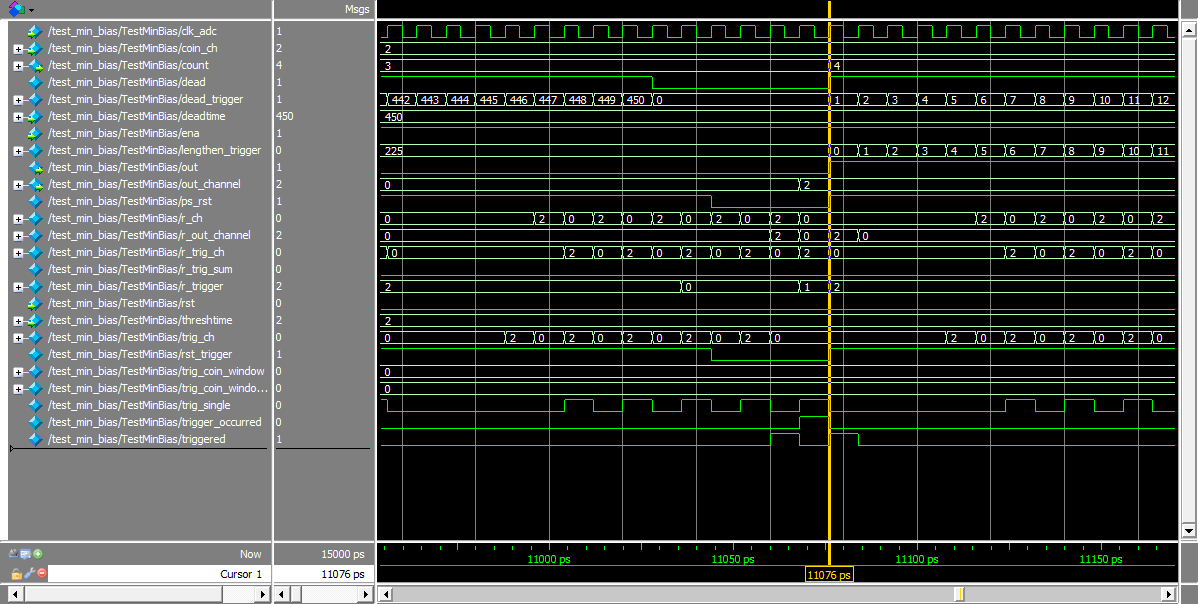
\includegraphics[width = \paperwidth]{minBiasSingleChannel.png}
	\caption{Timing diagram for the minimum bias trigger in single channel mode.}
	\label{Fig:minBiasSingleSim}
	\end{figure}
	\vspace*{\fill}
\end{landscape}

\begin{landscape}
\vspace*{\fill}
	\begin{figure}[ht]
	\centering
	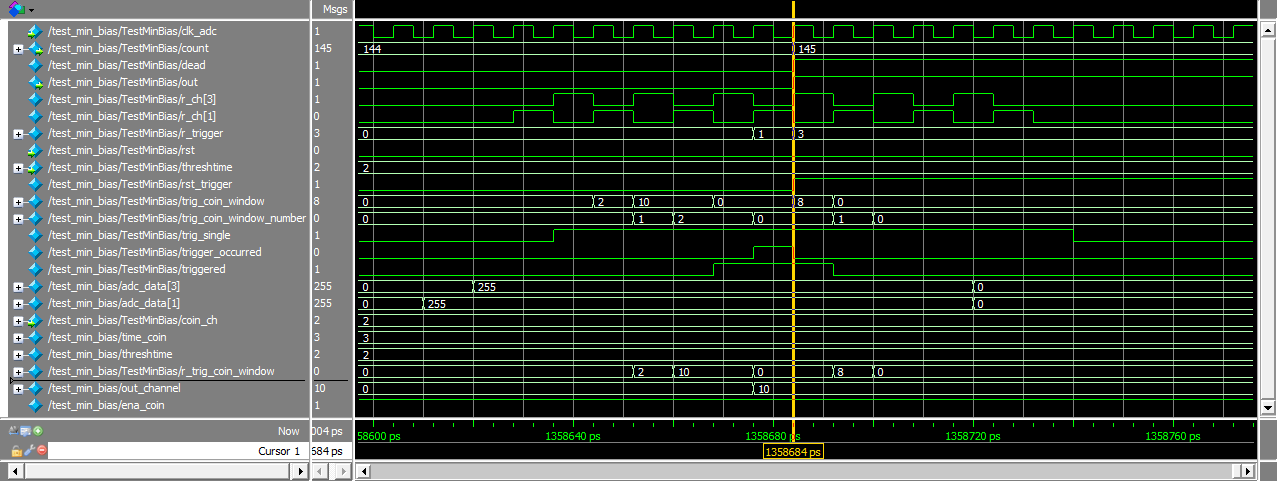
\includegraphics[width = \paperwidth]{minBiasCoincidence.png}
	\caption{Timing diagram for the minimum bias trigger in coincidence mode.}
	\label{Fig:minBiasCoincSim}
	\end{figure}
\vspace*{\fill}
\end{landscape}

\subsection{ODB Settings}
\label{sec:minBiasODB}
\begin{figure}[ht]
\centering
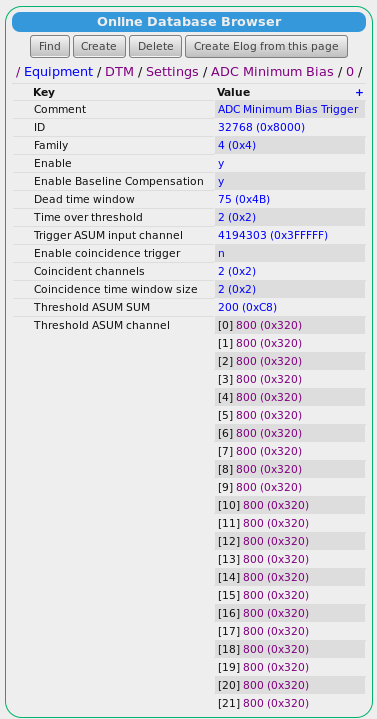
\includegraphics[height = 0.75\paperheight]{minBiasODB}
\caption{Online data base settings for the min. bias trigger.}
\label{Fig:minBiasODB}
\end{figure}

\begin{description}
\item \textbf{Trigger ID: } 0x8000

\item \textbf{Family: } 0x4 (Physics)

\item \textbf{Enable: }Turns the trigger module on/off

\item \textbf{Enable Baseline Compensation: }Will apply the baseline subtraction from the read ADC value. If enabled the thresholds will be used on the baseline subtracted reading.

\item \textbf{Dead Time Window: } 16-bit value which sets the number of clocks after a trigger event wherein no more triggers will be produced to avoid retrieving on the same event. (\NOTE{This should be significantly larger than the long time window}

\item \textbf{Time over Threshold: }16-bit value which sets the minimum number of clocks after a threshold has been crossed that the signal must remain high for a trigger to be produced. \NOTE{As this is used to only remove noise, the \gls{tot} is usually set at a only a few clocks}
 
\item \textbf{Trigger \gls{asum} input channel: } Bit mask for enabled channel inputs; a disabled channel has its corresponding bit set false. Bits 1-22 are the \gls{asum} channels and bit 23 is the \gls{ass}. Any combination can be enabled. 

\item \textbf{Coincident Channels: }Number of channels required to have fulfilled the triggering requirements within the coincident time window size if the coincidence trigger is enabled. For instance if this value is set to four, than within the coincidence time window size a minimum of 4 channels must have crossed their thresholds for a time greater than the \gls{tot} for a trigger to be produced.
	
\item \textbf{Coincident time window size: } 16-bit value which sets the number of clocks in the time window for the number of channels defined by the coincident channels setting to have each meant the single channel trigger requirements (only applies for coincidence trigger mode). 

\item \textbf{Threshold \gls{ass}: }17-bit value setting the minimum bias threshold for the \gls{ass}.

\item \textbf{Threshold \gls{asum} channel: }12-bit value setting the minimum bias threshold for each of the \gls{asum} channels.
\end{description}


\clearpage
\section{ADC Trigger}
\label{sec:adcTrig}
\begin{description}
\item[SVN Location: ]https://edev.triumf.ca/svn/edevel00261/trunk/tsb/ip/rtl/source/ts\_adc.v
\item[Module Name: ]TriggerSourceADC
\item[Frequency Range: ]Settings Dependant, minimum time between triggering five clock delay (reset and flip-flop setting) + dead time + scan time\footnote{Scan time in the \gls{odb}, look ahead time in the literature, the firmware variable in the timing diagram is 'waittime'} (See Fig. \ref{Fig:adcSim})
\item[Submodules: ]trigger\_self\_sum\_adc (see Section \ref{sec:selfSum}), TriggerSelfDecision (see Section \ref{sec:trigSelfDecision})
\item[Summary: ]The ADC trigger receives the baseline subtracted \gls{ass} and analyzes the short energy and \gls{fprompt} to make a triggering decision. The module trigger\_self\_sum (Section \ref{sec:selfSum}) performs a rolling integral over a short ($\sim$8 clocks)\footnote{This module uses the ADC clock of 45.161290 MHz} and a long time window ($\sim$150 clocks) as shown in Fig. \ref{Fig:adcTrigger}. The short integration window integral is delayed to be valid at the same time as the long window (see Section \ref{sec:selfSum}) so the decision is always made after the integration of both windows is finished.

The integrals are passed to the module TriggerSelfDecision (Section \ref{sec:trigSelfDecision}) which dynamically sorts 'events' into one of six groups as shown in Fig. \ref{Fig:triggerRegions}. If the charge in the short window exceeds the low energy limit, then a variable 'trig\_out' is set as shown in Fig. \ref{Fig:bitFieldADCTrig} (colours and bit positions are consistent with Fig. \ref{Fig:triggerRegions}). If the value of trig\_out increase (i.e. higher \gls{fprompt} or short charge) or stays the same with the energy increasing, the values from that time are saved and the comparison continues. If The value of trig\_out decreases or stays the same with the short energy decreasing or staying the same, then an \gls{odb} defined timer referred to as the look ahead time \footnote{this is called the scan time in the \gls{odb}, waittime in the firmware, or look ahead time in some documentation} ($\sim$15 clocks) begins counting. If a value of trig\_out of the same or greater value is found within this look ahead time, then that the values (short/long window charge, trigger type, and trigger start time, etc.) are set to the new events and the timer is restarted\footnote{If a second maxima is found in the look ahead time of equal or greater charge than the first, the scan time will start again from that point and the reported trigger will be of the last maxima.}. Only once the timer reaches the look ahead time without finding a higher value of trig\_out is a trigger produced.

\begin{figure}[ht]
\centering
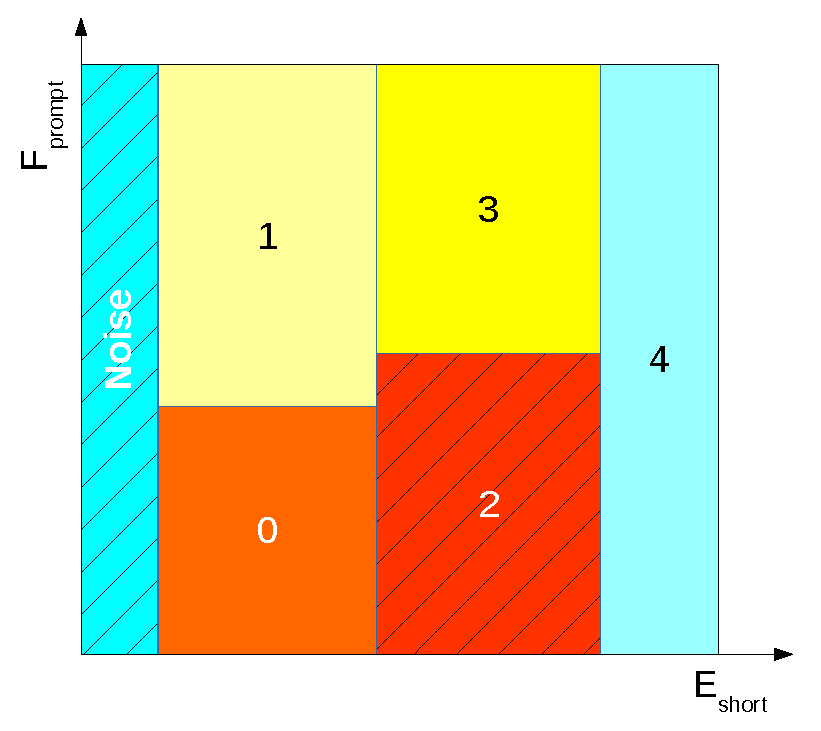
\includegraphics[width = 0.6\paperwidth]{triggerRegions}
\caption{Trigger regions as used in the pulse shape discrimination background rejection method. Noise in the \gls{pmt}s fall under very low energy and $\beta$ events are grouped into high energy, low \gls{fprompt}. The \gls{wimp} region of interest is at high \gls{fprompt} and could fall into either region of energy.}
\label{Fig:triggerRegions}
\end{figure}

\definecolor{orange}{rgb}{1.8,1,.1}
\begin{figure}
	\begin{bytefield}[endianness=big, bitheight=3.0\baselineskip]{30}
	\colorbitbox{webblue}{6}{Very High\\Energy\\Bit 4}
	\colorbitbox{yellow}{6}{High Energy\\High Fprompt\\Bit 3}
	\colorbitbox{red}{6}{High Energy\\Low Fprompt\\Bit 2}
	\colorbitbox{orange}{6}{Low Energy\\High Fprompt\\Bit 1}  
	\colorbitbox{webred}{6}{Low Energy\\Low Fprompt\\Bit 0}
	\end{bytefield}
	\caption{trig\_out variable, the higher the charge and \gls{fprompt}, the higher the value. Values and colours correspond to the regions shown in Fig. \ref{Fig:triggerRegions}.}
	\label{Fig:bitFieldADCTrig}
\end{figure}

\end{description} 
\begin{figure}[ht]
\centering
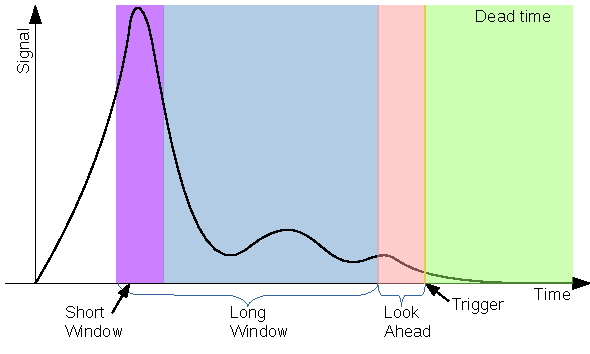
\includegraphics[width = 0.7\paperwidth]{adcTrigger}
\caption{Short and long time integration windows for the determination of the fraction of prompt charge in an event (\gls{fprompt}).}
\label{Fig:adcTrigger}
\end{figure}

The \gls{fprompt} is not explicitly calculated however it is used for event selection; for a defined \gls{fprompt} (for 1$<$F$_{\text{thres}}< 256$) an event is recorded if:

\begin{equation}
\text{E}_{\text{long}} > \text{E}_{\text{thres}} \ \& \ \text{E}_{\text{long}} \times \text{F}_{\text{thres}} >\left[ \text{E}_{\text{short}} \times 256\right].
\label{Eq:fpromptDecision} 
\end{equation}
Thus if a \gls{fprompt} of 0.5 is desired, the \gls{odb} value is set to F$_{\text{thres}} = (256 \times 0.5) = 128$. Events are sorted using the short energy and \gls{fprompt} into one of five regions as depicted in Fig. \ref{Fig:triggerRegions} (region 0 is defined as below threshold therefore nothing is recorded).

After a trigger signal has been generated the trigger will enter a dead state where no triggering is allowed. This dead time is implemented so as to avoid retriggering on the same event\footnote{Note that the scan time adds to the dead time for the minimum time between triggers}. A diagram of the ADC trigger is given in Fig. \ref{Fig:adcTrigger}. 

\NOTE{The look ahead time does occur after the long window finishes integrating, but as the short and long window times are valid at the same time due to a delay fifo, the look ahead time applies 'back in time' if you will with regards to Fig. \ref{Fig:adcTrigger}}. A full timing diagram of the ADC trigger while constantly triggering is shown in Fig. \ref{Fig:adcSim}. 

\begin{landscape}
	\vspace*{\fill}
	\begin{figure}[ht]
	\centering
	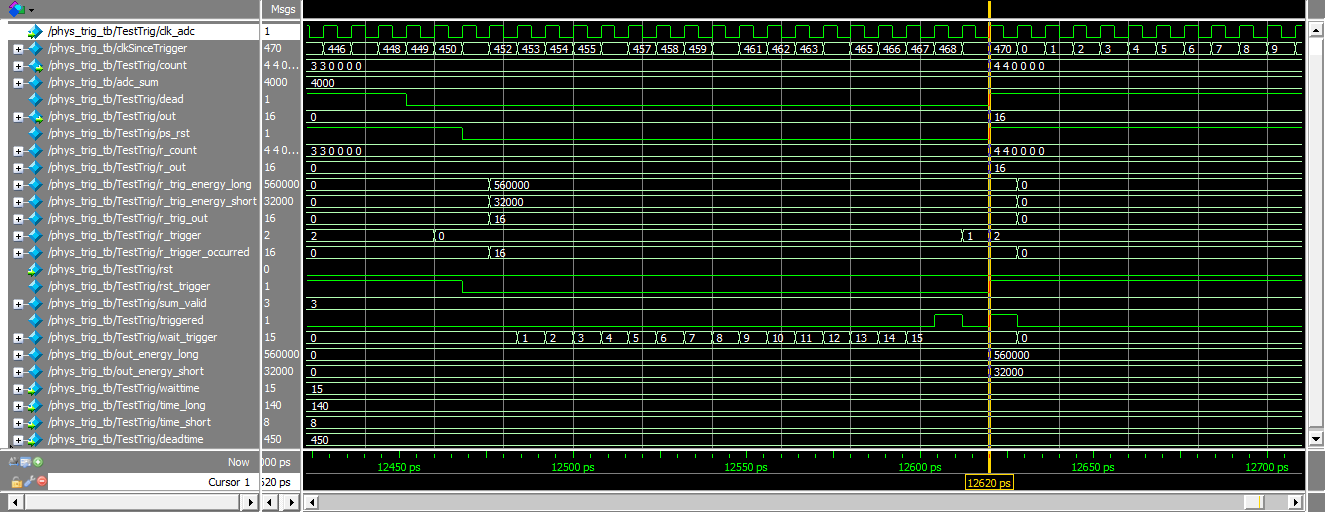
\includegraphics[width = \paperwidth]{adcTrigSim.png}
	\caption{Timing diagram for the ADC trigger at constant triggering.}
	\label{Fig:adcSim}
	\end{figure}
	\vspace*{\fill}
\end{landscape}


\subsection{ODB Settings}
\label{sec:adcTrigODB}
\begin{figure}[ht]
\centering
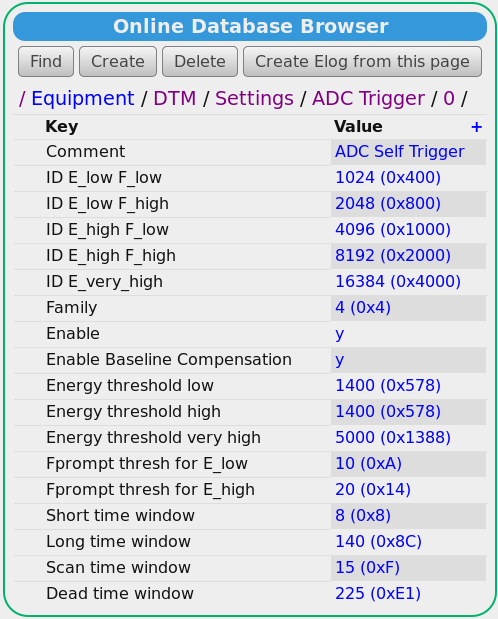
\includegraphics[width = 0.5\paperwidth]{adcTrigODB}
\caption{Online data base settings for the ADC trigger.}
\label{Fig:adcTrigODB}
\end{figure}

\begin{description}

\item \textbf{Trigger ID: } The ADC trigger has only a single channel but has 5 trigger IDs corresponding to the five zones depicted in Fig. \ref{Fig:triggerRegions}. These trigger types are taken from trig\_adc depicted in Fig. \ref{Fig:bitFieldADCTrig}.
	\begin{description}
	\item \textbf{Zone 0}: 0x400
	\item \textbf{Zone 1}: 0x800
	\item \textbf{Zone 2}: 0x1000
	\item \textbf{Zone 3}: 0x2000
	\item \textbf{Zone 4}: 0x4000
	\end{description}

\item \textbf{Family: }0x4 (Physics)

\item \textbf{Enable: }Turns the trigger module on/off

\item \textbf{Enable Baseline Compensation: }Will apply the baseline subtraction from the read ADC value. If disabled the thresholds will be used on the baseline subtracted reading. \NOTE{The \gls{fprompt} is nonsensical with this disabled.}

\item \textbf{Energy Thresholds: }17-bit value (sum of 22 12-bit \gls{asum}s). If the baseline subtraction is enabled then the thresholds are taken from the subtracted reading.
	\begin{description}
	\item \textbf{Low: }Cutoff between noise and zones 0/1
	\item \textbf{High: }Cutoff between zones 0/1 and zones 2/3
	\item \textbf{Very High: }Cutoff between noise zones 2/3 and zone 4 
	\end{description}

\item \textbf{\gls{fprompt} Thresholds: }Cutoff between low and high \gls{fprompt}. \gls{fprompt} is given as an eight bit value, trigger decisions follow Eq. \eqref{Eq:fpromptDecision}.
	\begin{description}
	\item \textbf{Low Energy: }\gls{fprompt} separation between zones 0 and 1
	\item \textbf{High Energy: }\gls{fprompt} separation between zones 2 and 3
	\end{description} 
	
\item \textbf{Short Time Window: } 1-50 value (1.1 $\mu$s) which sets the number of clocks the charge in the short integration window (see Fig. \ref{Fig:adcTrigger})

\item \textbf{Long Time Window: }1-500 value (11 $\mu$s) which sets the number of clocks the charge in the long integration window (see Fig. \ref{Fig:adcTrigger})

\item \textbf{Scan Time Window: }16-bit value which sets the number of clocks to look to see if the currently found maxima is local or general (within the scan time). The scan time is intended to ensure that the integrated value of the short window is maximized.

\item \textbf{Dead Time Window: }16-bit value which sets the number of clocks after a trigger event wherein no more triggers will be produced to avoid retriggering on the same event. \NOTE{This should be significantly larger than the long time window.}

\end{description}

\section{ODB}
\label{sec:odb}
The online data base (\gls{odb}) contains all of the controls and settings for the triggers on a webpage. More information on the \gls{odb} can be found \hypNote{on the \gls{midas} site}{https://midas.triumf.ca/MidasWiki/index.php/Online_Database}.


The \gls{dtm} \gls{odb} settings can be found in their entirety on the \hypNote{twiki}{https://www.snolab.ca/deap/private/TWiki/bin/view/Main/Dtmodb}

\chapter{Firmware Modules $\&$ Settings}
\label{chap:firmware}

\section{SVN Structure}

The SVN structure used for the \gls{deap3} firmware depicted in Fig. \ref{Fig:firmHier} has two main logical parts, the physics payload (red) and the \gls{fmc} drivers/software (blue) combined as SVN externals to the top project (green). 
The modules pertaining to the function of the trigger is considered the physics payload and is made up of  edevel00261 (Section \ref{sec:261}), edevel00260 (see Section \ref{sec:260}), and parts of edevel00270 (Section \ref{sec:270}). 
The rest of the drivers and control code is apart from the trigger itself and is beyond the scope of this manual. 
For more specifics on the driver firmware look at the repository\footnote{\url{https://edev.triumf.ca/project/deap/edevel00013}}, or contact Yair Linn\footnote{yairlinn@triumf.ca} or Daryl Bishop\footnote{daryl@triumf.ca}. The firmware pertaining to the trigger and general operation of the \gls{dtm} follow.

\begin{landscape}
	\vspace*{\fill}
	\begin{figure}[ht]
	\centering
	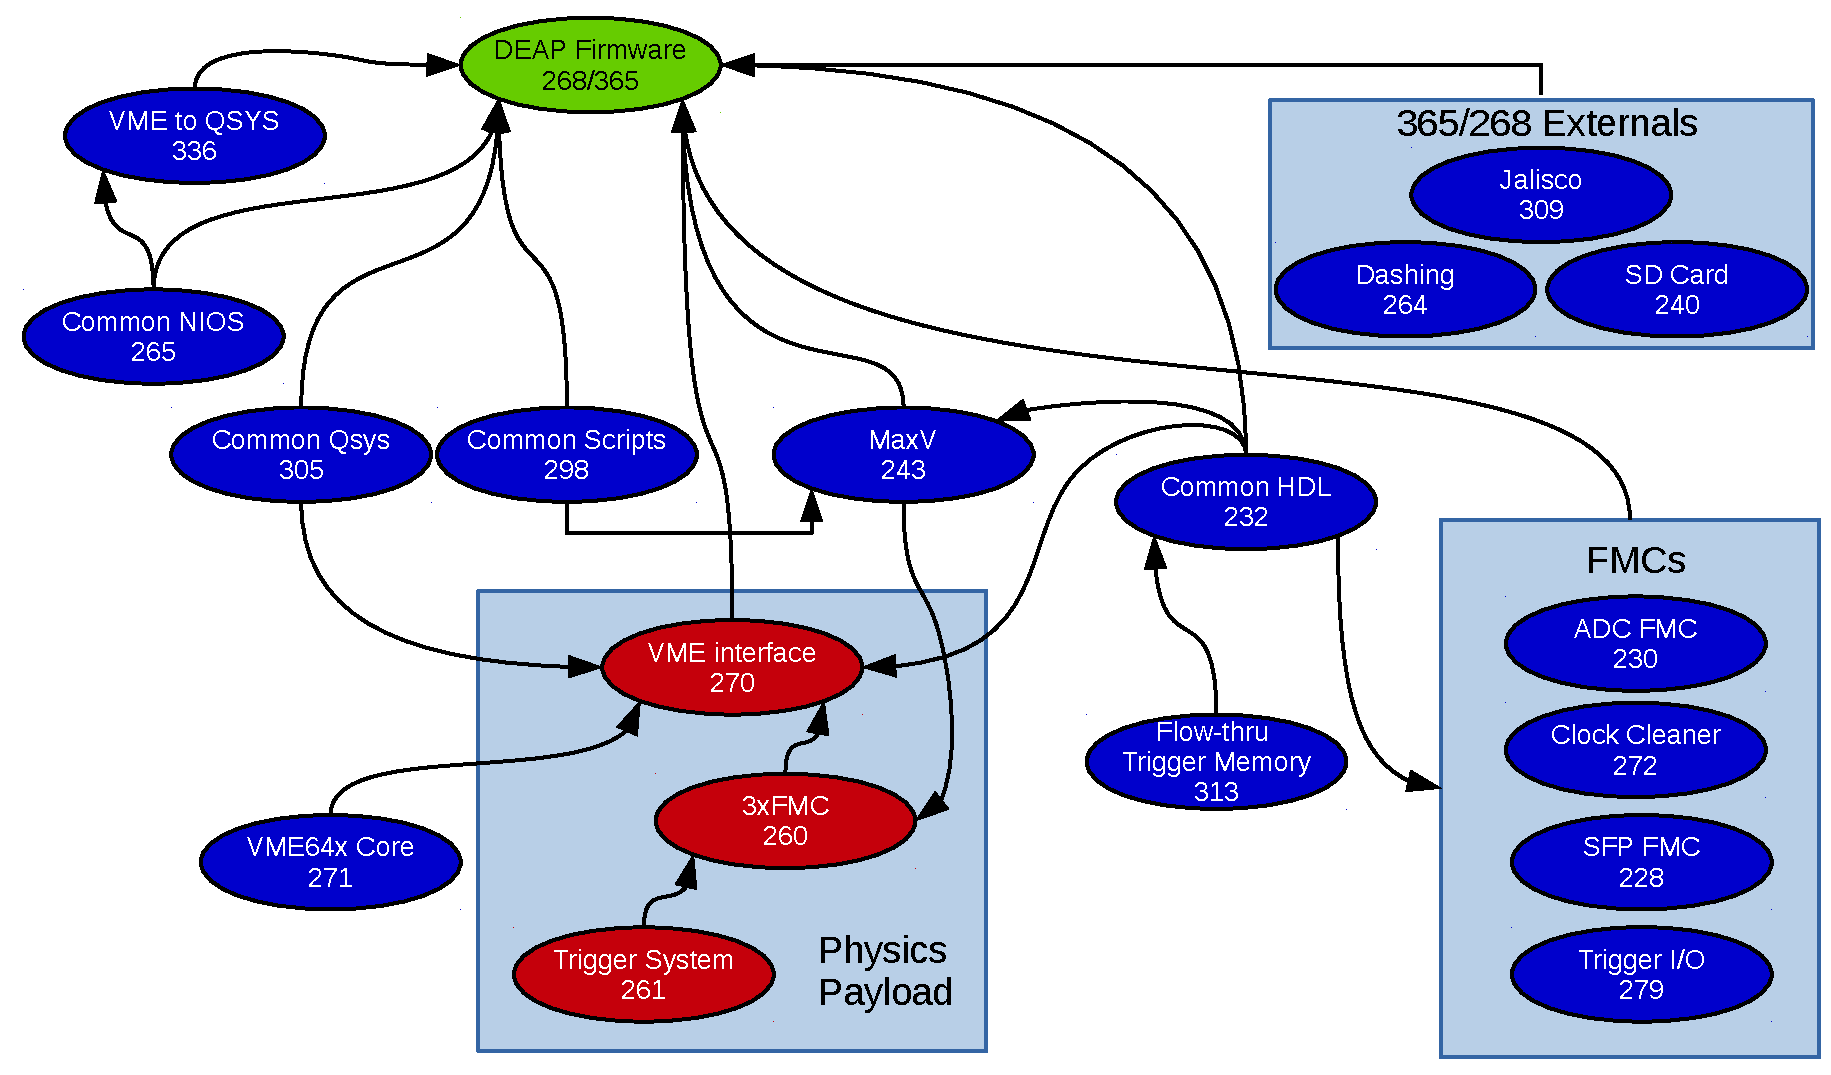
\includegraphics[width = .73\paperheight]{firmwareHier}
	\caption{Flow chart of the firmware SVN structure. The top project is either edevel00268 or edevel00365 with the various other projects connected as externals. The modules in blue are maintained by the TRIUMF EDEV department whereas the modules in red (the physics payload) is maintained by \gls{deap3}. The externals for 268 and 365 are identical as shown.}
	\label{Fig:firmHier}
	\end{figure}
	\vspace*{\fill}
\end{landscape}


\section{Trigger System (edevel00261)}
\label{sec:261}
\begin{description}
\item[SVN Location:] https://edev.triumf.ca/svn/edevel00261
\item[Last Installed Tag:] \tagTwoSixOne %this is defined in triggerManual.tex at the start of the document
\item[Externals:] None
\item[Summary:] The trigger system code contains all of the trigger modules and submodules which are called into the \gls{vme} interface (Section \ref{sec:270}). All the trigger modules described in Chapter \ref{chap:triggers} are located in tsb/ip/rtl/source. The other trigger system modules are introduced below.
\end{description}
	

	
	\subsection{Baseline Compensation}
	\label{sec:baseline}
	\begin{description}
	\item[Module Name:] trigger\_baseline
	\item[SVN Location:] \url{https://edev.triumf.ca/svn/edevel00261/trigger\_baseline.v}
	\item[Modules used in:] ts\_adc $\&$ min bias, deap\_vme\_interface\_wrapper.v 
	\end{description}
	
	
	\begin{figure}[ht]
	\centering
	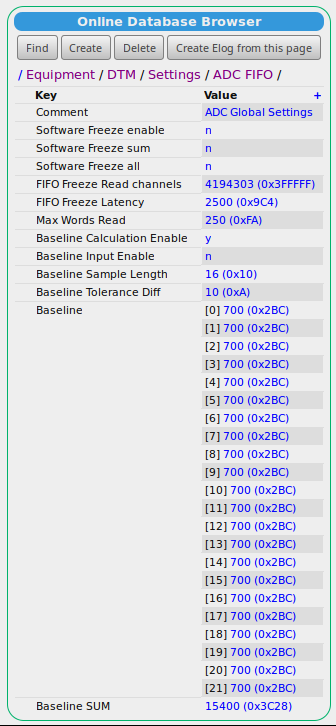
\includegraphics[height = .8\paperheight]{adcFIFO}
	\caption{Online data base settings for the ADC FIFO and baselines.}
	\label{Fig:adcFIFO}
	\end{figure}
	
	
	The ADC baseline compensation module is a module designed for the ADC trigger (Section \ref{sec:adcTrig}) source to allow the calculation of \gls{fprompt}. The minimum bias trigger (Section \ref{Fig:minBiasTrigger}) is also configured for it, but there is little motivation to use it as absolute ADC threshold values are equivalently useful.
	
	The baseline calculation is preformed with an averaging function that sums ADC data (each \gls{asum} channel has its own compensation module) for 2$^n$ bins (the value of n is set in the \gls{odb}, a common value is 16 bins, i.e. n = 4). The sum is then right shifted by n bits giving the average value of the 2$^n$ bins.
	A default value is set in the \gls{odb} and is used as the starting baseline. This value can remain static, an external baseline can be inputed, or a dynamic calculation can be enabled.
	
		\subsubsection{Baseline Calculation}
		
		If placed in baseline calculation mode as is typical to allow for some drift as is expected from the PMTs, the baseline will dynamically calculated and adjusted. Every 2$^n$ clocks the baseline is re-averaged in the manner described above. This new value is compared to the previously set baseline and the difference is recorded. This repeats with the difference between the set and re-averaged baselines being summed each time. If the difference exceeds the tolerance set in the \gls{odb} then the set baseline is incremented by one in the direction of the trend. If the difference exceeds the tolerance the set baseline is incremented by one as the baseline is tending low. If the difference is less than the negative tolerance, the set baseline is decremented by one as the baseline is tending high.
		
		The algorithm starts to run after the DTM is booted, so before the start of the run. However, it is reset at each start of run by the frontend. The baselines of all channels are not currently\footnote{July, 2016} saved into the data structure, however the long term stability can be seen on the front end.
		
		Although previously the \gls{ass} baseline was calculated as the sum of the \gls{asum} baselines (as stated in the twiki\footnote{\url{https://www.snolab.ca/deap/private/TWiki/bin/view/Main/DTMBaseline}} location), this baseline is calculated separately from the sum of the signals.
		
		\NOTE{The change of the \gls{ass} baseline calculation is to remove the offset caused by truncation, with 22 channels the truncation error would average 11 ADC off.}

		\subsubsection{Baseline Stability}
		\begin{description}
		\item[\gls{odb} Baseline Plot: ]\url{https://deapdaqgw.snolab.ca/HS/Baseline/}	
		\end{description}
		The baseline values are not currently\footnote{July, 2016} readout into the RAT data structure, however the stability can be monitered online at the location given above. Each of the \gls{asum} baselines (Fig. \ref{Fig:baselineStabilityAsum1}  and Fig. \ref{Fig:baselineStabilityAsum2} ) are monitered as well as the \gls{ass} (Fig. \ref{Fig:baselineStability}). 
		
		\NOTE{The three day monitering is shown in Fig. \ref{Fig:baselineStabilityAsum1} - \ref{Fig:baselineStability} but this plot goes from 10 min to 7 days and of course can be configured to other times.}
		
		\begin{figure}[ht]
		\centering
		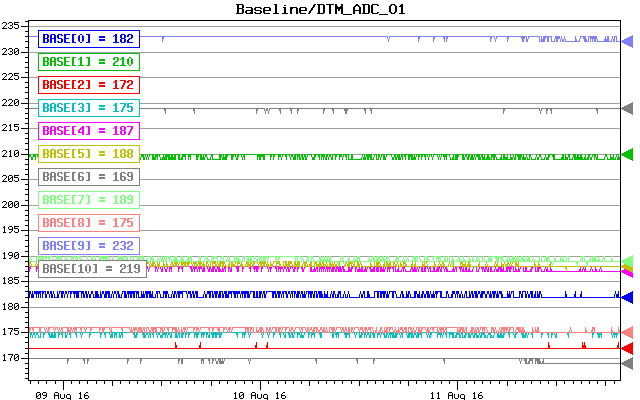
\includegraphics[width = .8\textwidth]{DTM_ADC_01}
		\caption{Long time plot of the first 11\gls{asum} baselines over a 3 day period. Each baseline is continuously calculated and allowed to change.}
		\label{Fig:baselineStabilityAsum1}
		\end{figure}		
		
		\begin{figure}[ht]
		\centering
		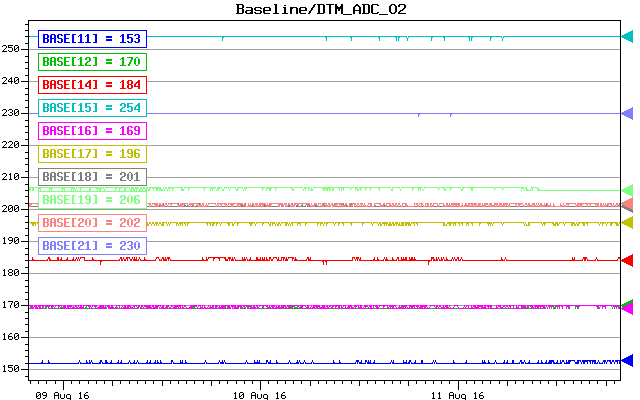
\includegraphics[width = .8\textwidth]{DTM_ADC_02}
		\caption{Long time plot of \gls{asum}s 11-21 baselines over a 3 day period. Each baseline is continuously calculated and allowed to change.}
		\label{Fig:baselineStabilityAsum2}
		\end{figure}
						
		\begin{figure}[ht]
		\centering
		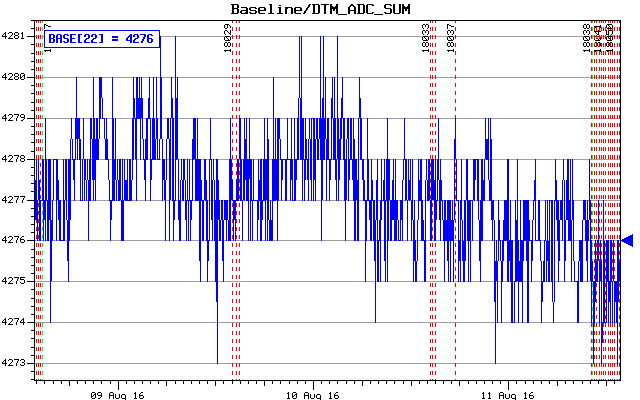
\includegraphics[width = .8\textwidth]{baselineStability}
		\caption{Long time plot of the \gls{ass} baseline over a 3 day period. The baseline is continuously calculated and allowed to change.}
		\label{Fig:baselineStability}
		\end{figure}		
						
	
	\clearpage
	\subsection{Self Sum Module}
	\label{sec:selfSum}
	\begin{description}
	\item[Module Name:] trigger\_self\_sum\_adc
	\item[SVN Location:] tsb/ip/rtl/trigger\_self\_sum\_adc.v
	\item[Modules used in:] TriggerSourceADC
	\item[Summary:] Returns the integrated charge within a defined short and long time window of the baseline subtracted (see above) \gls{ass} continuously. Both integrations start at the same time, so the short time window result is held in a FIFO with respect to the end of the long time window so that both results are present at the same time. The maximum values for windows are 50 \gls{dtm} clocks for the short window (TICKS\_SHORT = 50) and 500 \gls{dtm} clocks for the long window (TICKS\_LONG = 500). At 22.14 ns these max times are 1107 ns and 11070 ns respectively. %Clock domain change from ADC clock (45.161290 MHz) to DAQ clock (62.5 MHz) is provided using FIFOs.
	\end{description}
	
	
	\subsection{Trigger Self Decision Module}
	\label{sec:trigSelfDecision}
	\begin{description}
	\item[Module Name:] TriggerSelfDecision
	\item[SVN Location:]  tsb/ip/rtl/trigger\_self\_decision.v
	\item[Modules used in:] TriggerSourceADC
	\item[Summary:] The self decision module uses the short and long integrated \gls{ass} windows passed by the trigger\_self\_sum\_adc module (See above). As described in Section \ref{sec:adcTrig} and shown in Fig. \ref{Fig:triggerRegions} there are 4 energy regions: very low (or noise), low, high, and very high with the low and high regions being separated by their \gls{fprompt}. Energy selection is done by simply comparing the set threshold to the short energy from the self sum module. The energy is sorted into very high, then high, then low. The \gls{fprompt} selection is done by left shifting the short charge by eight bits and comparing that value to the \gls{fprompt}s for each region (as set in the \gls{odb} as a value [1-256]) multiplied by the long window charge. The highest energy followed by highest \gls{fprompt} is set first.
	\end{description}
	
	\subsection{Trigger Top Module}
	\label{sec:trigTop}
	\begin{description}
	\item[Module Name:] DEAPTriggerTop
	\item[SVN Location:]  tsb/ip/rtl/trigger\_top.v
	\item[Modules used in:] vme wrapper
	\item[Summary: ]Trigger top level module. Calls TriggerNIMIO, TriggerEventArbiterWithFIFO, and TriggerPrescalerWithFIFO. This module looks after what happens after one of the enabled triggers puts out a signal, contains the NIM output control. Runs on the 62.5 MHz \gls{daq} clock. Prescales events and takes care of collisions of events in TriggerEventArbiterWithFIFO. The event data written to the arbiter \gls{fifo} is passed to VME\_MAPPED\_REGFILE\_STATUS which is then read out by \gls{midas}. 
	
	\NOTE{It was being talked about adding a shutdown if events come too quickly, that could either be done here or in TriggerEventArbiterWithFIFO.}	
	\end{description}	
	
		\subsubsection{Trigger Event Arbiter With FIFO}
		\label{sec:triggerEventArbiterWithFIFO}
		\begin{description}
		\item[Module Name:] TriggerEventArbiterWithFIFO
		\item[SVN Location:]  tsb/ip/rtl/trigger\_event.v
		\item[Modules used in:] DEAPTriggerTop
		\item[Summary:] Deals with what event from the prescalers gets sent through and written to a \gls{fifo}. Reads through events in prescalers by Round Robin Arbitration (One clock cycle per prescaler). Checks all the other prescalers if an event with the same timestamp is available if they are then they are merged if not, but another event with an earlier timestamp is available, buffer the first event and go to the earlier one. If no other event with the same or earlier timestamp is available then the event is written to the \gls{fifo}. This method ensures that although there are several different triggers, the ones written out to \gls{midas} are all is sequential order.
		
		\NOTE{It was being talked about adding a shutdown if events come too quickly, that could either be done here or in DEAPTriggerTop.}
		\end{description}
	
		\subsubsection{Trigger Prescaler With FIFO}
		\label{sec:trigPrescaleFifo}
		\begin{description}
		\item[Module Name:] TriggerPrescalerWithFIFO
		\item[SVN Location:]  tsb/ip/rtl/trigger\_prescaler\_fifo.v
		\item[Modules used in:] DEAPTriggerTop
		\item[Summary:] Calls TriggerPrescaler and writes a \gls{fifo} with all of the trigger information for readout by TriggerEventArbiterWithFIFO. The trigger information is saved in a \gls{fifo} until called. Each trigger type has its own \gls{fifo} of nominally 16 words deep. If the module receives a trigger it will write the trigger information to the \gls{fifo} and the sequential events will be readout by the arbiter.
		\end{description}
		
		
		\subsubsection{Trigger Prescaler}
		\label{sec:trigPrescaler}
		\begin{description}
		\item[Module Name:] TriggerPrescaler
		\item[SVN Location:]  tsb/ip/rtl/trigger\_prescaler.v
		\item[Modules used in:] TriggerPrescalerWithFIFO
		\item[Summary:] Counts the number of triggers that come in and output one once the set prescale amount is met. Syncs the various event builder data so that the output of the trigger is valid with the values of the short/long ADC integrated charge or the number of coincidence channels from the Min. bias trigger. 
		\end{description}
	

		\subsubsection{Trigger NIM I/O}
		\label{sec:triggerNIMIO}
		\begin{description}
		\item[Module Name:] TriggerNIMIO
		\item[SVN Location:]  tsb/ip/rtl/trigger\_nim\_io.v
		\item[Modules used in:] DEAPTriggerTop
		\item[Summary:] Trigger output module. This module receives a trigger signal in for one of its 8 output channels. The module checks to see if the suppression time since the last output on that channel has been exceeded yet, if it has and the busy signal is false the trigger count for that channel is incriminated and a trigger signal is sent out of the designated output. If the busy input on the NIM I/O \gls{fmc} is high then no trigger output can occur\footnote{For more on the busy signals see the twiki: \url{https://www.snolab.ca/deap/private/TWiki/bin/view/Main/InfoBusy}}.
		\end{description}
	

	
\section{3xFMC (edevel00260)} 
\label{sec:260}
\begin{description}
\item[SVN Location:] https://edev.triumf.ca/svn/edevel00260
\item[Last Installed Tag:] \tagTwoSixZero %this is defi/tsbs/deap_vme_and_daq/tsbs/trigger_and_daq/ned in triggerManual.tex at the start of the document
\item[Externals:] MaxV (edevel00243), TriggerSystem (edevel00261) 
\item[Summary:] Contains the NIOS core for the exponential trigger, the software which generates the exponential random number and the global parameters used in the trigger system (parameters.v).
\end{description}
\NOTE{Contains the global parameters for the trigger system in parameters.v}

\section{DEAP VME Interface (edevel00270)} 
\label{sec:270}
\begin{description}
\item[SVN Location:] https://edev.triumf.ca/svn/edevel00270
\item[Last Installed Tag:] \tagTwoSevenZero %this is defi/tsbs/deap_vme_and_daq/tsbs/trigger_and_daq/ned in triggerManual.tex at the start of the document
\item[Externals:] Common QSYS (edevel00305), Common HDL (edevel00232), VME64x Core (edevel00271), 3xFMC (edevel00260)
\item[Summary:] The VME Interface is the top SVN project of the physics payload as shown in Fig. \ref{Fig:firmHier}. Although not containing any of the actual \gls{fmc} drivers themselves, this project encapsulates all of the data taking and processing as well as all of the triggers and event selection.
\end{description}

	\subsection{VME Interface Wrapper} 
	\label{sec:vmeWrapper}
	\begin{description}
	\item[Module Name:] deap\_vme\_interface\_wrapper
	\item[SVN Location:]  tsb/ip/rtl/deap\_vme\_interface\_wrapper.v
	\item[Modules used in:] VME\_3xFMC\_Carrier (edevel00365 or edevel00268 in tsb/ip/rtl/VME\_3xFMC\_Carrier.v)
	\item[Summary: ]This is the top level verilog file of this subproject. Instantiates the DEAP trigger sources, ADC \gls{vme} \gls{fifo}s, \gls{deap} trigger top module, exponential trigger NIOS, \gls{vme} registers and their assignments. Anything related to the ADC Waveform FIFOs is to be done in this file. This module contains all of the physics level firmware.
	\end{description}

	

\section{DEAP Firmware Development Quartus 13.0sp1 (edevel00268)} 
\label{sec:268}
\begin{description}
\item[SVN Location:] https://edev.triumf.ca/svn/edevel00268
\item[Last Installed Tag:] \tagTwoSixEight %this is defined in triggerManual.tex at the start of the document
\item[Externals:]  \gls{jalisco} (edevel00309), Dashing (edevel00264), SD Card (edevel00240), VME to QSYS (edevel00336), MaxV (edevel00243), Common NIOS (edevel00265), Common QSYS (edevel00305), Common Scripts (edevel00298), Common HDL (edevel00232), ADC FMC (edevel00230), Clock Cleaner (edevel00272), SFP FMC (edevel00228), Trigger I/O (edevel00279), VME Interface (edevel00270)
\item[Summary: ]Currently edevel00268 is the top SVN project for \gls{deap3}. Each of the preceding files and projects described above (excluding edevel00268) are included as externals. 268 uses the master clock distribution \gls{fmc} board (see Section \ref{sec:mClockBoard}) with daisy chain clocking. 268 has experienced issues operating on the 3xFMC Rev. A board and therefore is only used with the Rev. B board (See the Errata \ref{chap:errata}). See Section \ref{sec:dtmConfigs} for the applicable hardware configuration. The programming scripts for the FPGAs are located in tsb/ip/scripts\footnote{see Chapter \ref{chap:install} for programming} with the binary files to be loaded held in tsb/ip/exe.

\NOTE{It is crucial to make sure the correct \gls{fmc}s are connected, \textbf{do not} load 268 with the SFP and Mini-Sas board attached and \textbf{do not} load 365 with the Clock distribution \gls{fmc}.} 
\end{description}

	\subsection{VME 3xFMC Carrier} 
	\label{sec:VME_3xFMC_Carrier268}
	\begin{description}
	\item[Module Name:] VME\_3xFMC\_Carrier
	\item[SVN Location:]  tsb/ip/rtl/VME\_3xFMC\_Carrier.v
	\item[Modules used in:] N/A (Top Project Module)
	\item[Summary: ]This is the very top module of the \gls{deap3} firmware, and instantiates the deap\_vme\_interface\_wrapper module. This module is maintained exclusively by Yair Linn\footnote{yairlinn@triumf.ca}.
	\end{description}


\section{DEAP Firmware Quartus 14.1 (edevel00365)}
\label{sec:365}
\begin{description}
\item[SVN Location:] https://edev.triumf.ca/svn/edevel00365
\item[Last Installed Tag:] \tagThreeSixFive %this is defined in triggerManual.tex at the start of the document
\item[Externals:]  \gls{jalisco} (edevel00309), Dashing (edevel00264), SD Card (edevel00240), VME to QSYS (edevel00336), MaxV (edevel00243), Common NIOS (edevel00265), Common QSYS (edevel00305), Common Scripts (edevel00298), Common HDL (edevel00232), ADC FMC (edevel00230), Clock Cleaner (edevel00272), SFP FMC (edevel00228), Trigger I/O (edevel00279), VME Interface (edevel00270)
\item[Summary: ]Like edevel00268, edevel00365 is the top SVN project for \gls{deap3}, however the upgrade has not yet occurred\footnote{Upgrade date as yet unset (as of July 2016)}. Each of the preceding files and projects described above (excluding edevel00268) are included as externals. 365 uses the SFP and Mini-Sas \gls{fmc} board (see Section \ref{sec:SFPBoard}) adding FTP connectivity to the \gls{dtm} (see Chapter \ref{chap:install}). Additionally 365 has tighter timing constraints which has fixed the issues experienced with using 268 on the 3xFMC Rev. A board so may operate on either board (See the Errata \ref{chap:errata}). See Section \ref{sec:dtmConfigs} for the applicable hardware configuration. The programming scripts for the FPGAs are located in tsb/ip/scripts\footnote{see Chapter \ref{chap:install} for programming} with the binary files to be loaded held in tsb/ip/exe.

\NOTE{It is crucial to make sure the correct \gls{fmc}s are connected, \textbf{do not} load 268 with the STP and Mini-SAS board attached and \textbf{do not} load 365 with the clock distribution \gls{fmc}.} 

	\subsection{VME 3xFMC Carrier} 
	\label{sec:VME_3xFMC_Carrier365}
	\begin{description}
	\item[Module Name:] VME\_3xFMC\_Carrier
	\item[SVN Location:]  tsb/ip/rtl/VME\_3xFMC\_Carrier.v
	\item[Modules used in:] N/A (Top Project Module)
	\item[Summary: ] This is the same module as used in edevel00268 with several significant changes. This module is maintained exclusively by Yair Linn\footnote{yairlinn@triumf.ca}.
	\end{description}
	
\end{description}

%\include{software}
\chapter{Installation and Operation}
\label{chap:install}
\section{JALISCO}
\label{sec:jalisco}
\begin{description}
\item[EDEV Project:] \url{https://edev.triumf.ca/projects/edevel00309}
\item[EDEV Wiki:] \url{https://edev.triumf.ca/projects/edevel00309/wiki}
\item[Tutorial Videos:] \url{https://edev.triumf.ca/projects/edevel00365/wiki/Jalisco_Tutorial_Videos}
\end{description}
The Java Lightweight System Console, or \gls{jalisco}, is a Java based GUI that controls most aspects of the \gls{dtm} hardware boards. Currently used in various projects such as \gls{deap3}, \gls{jalisco} is unique in that it automatically generates its GUI based on the autodiscovery of the register files inside the firmware. So if the register exists in the firmware, it can be readout and altered by \gls{jalisco}.

\gls{jalisco} adds a GUI interface to the \gls{vme} readout for all read/write and read-only \gls{dtm} registers for the trigger and \gls{fmc}s. The ADC's can be read out directly, allowing debugging of any hardware issues separate from the firmware. See the wiki and the tutorial videos for more information. \gls{jalisco} is maintained by Yair Linn\footnote{yairlinn@triumf.ca}.

The \gls{jalisco} startup screen is shown in Fig. \ref{Fig:jaliscoTopScreen}. Once \gls{jalisco} is started and the appropriate host computer and port chosen, this GUI pops up. 
\begin{figure}[ht]
\centering
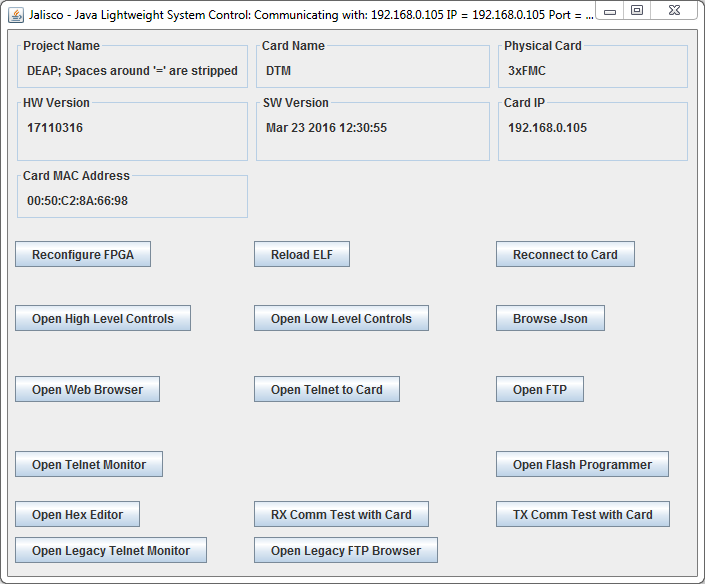
\includegraphics[width=.8\textwidth]{jaliscoTopScreen}
\caption{Main menu of \gls{jalisco} following startup.}
\label{Fig:jaliscoTopScreen}
\end{figure}

\clearpage

\section{Loading Firmware}
\NOTE{See the \href{https://edev.triumf.ca/projects/edevel00365/wiki/Boot_Sequence_and_Boot_Image_Selection}{EDEV page for more information.}}

\begin{figure}[ht]
\centering
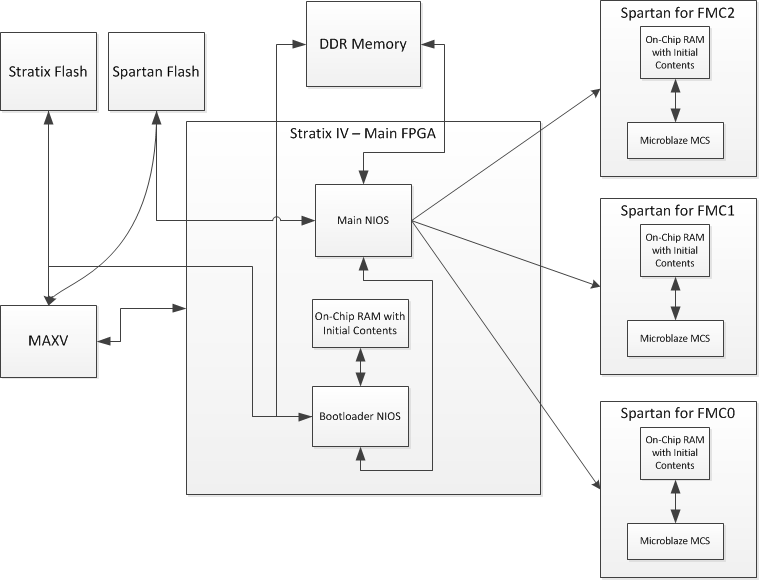
\includegraphics[width=\textwidth]{dtmDataStorage}
\caption{General layout of the FPGA, Embedded Processors, and Memory Devices on the \gls{dtm}. Photo Credit EDEV Department (\url{https://edev.triumf.ca/projects/edevel00365/wiki/Boot_Sequence_and_Boot_Image_Selection}).}
\label{Fig:dtmDataStorage}
\end{figure}

The installation of new firmware is done one of three different ways\footnote{To date (July 2016) only JTAG loading is used}: JTAG, FTP/Telnet, $\&$ via \gls{jalisco}. The safest method to update the firmware is over FTP. % FIXME (procedure outlined in Section \ref{sec:ftpLoading}). 
There are two versions of each flash image loaded as outlined in the following section (\ref{sec:dualImages}). Once the various FPGA images are loaded into the respective flash locations, the power is cycled loading the new firmware. 

\NOTE{Once a new image has been loaded check the \gls{jalisco} timestamp (see Section \ref{sec:jalisco})}

\subsection{Dual Load Images}
\label{sec:dualImages}
There are two images loaded onto the flash normally. The general concept is that there is a “normal image” or what should be used in normal operation and the image that is updated using \gls{jalisco} or FTP, and a “fallback image” that, for safety, cannot be modified via \gls{jalisco} nor FTP (only via JTAG) so it is far less susceptible to corruption. If an issue is detected with the primary image the secondary one will be used. 

There are three parts to a complete image load and it is crucial that the correct pairing of files is done.
\begin{enumerate}
\item Hardware (.pof) image of the Stratix FPGA
\item Software Image for the Main Nios (.elf)
\item Software and Hardware images for Spartans on FMC 0, FMC1, and FMC2 (.hex)
\end{enumerate}

Compiling of a new firmware release should be requested from the primary developer (Yair Linn\footnote{yairlinn@triumf.ca}).
The address map of the Stratix and the Spartan Flash images are shown in Fig. \ref{Fig:stratixImageFile} and \ref{Fig:spartanImageFile}.%\FIXME{WHAT IS THE TOP ADDRESS OF THESE?}.

\definecolor{lightgray}{gray}{0.8}
\begin{figure}
	\begin{bytefield}{12}
		\begin{rightwordgroup}{Stratix IV Dual Image}
			\memsection{0x0}{0x1000000}{3}{Page 0 - Normal Hardware Image (.pof)}\\
			\memsection{}{0x2000000}{3}{Normal Software Image (.elf)}\\
			\memsection{}{0x3000000}{3}{Page 1 - Fallback Hardware Image (.pof)}\\
			\memsection{}{0x3FFFFFF}{3}{Fallback Software Image (.elf)}
		\end{rightwordgroup}\\
	\end{bytefield}
	\caption{The address map of a Stratix IV flash file.}
	\label{Fig:stratixImageFile}
\end{figure}

\begin{figure}
	\begin{bytefield}{24}
		\begin{rightwordgroup}{Spartan-6 Dual Images}
			\memsection{0x0}{0x200000}{3}{FMC0 Normal Image}\\
			\memsection{}{0x400000}{3}{FMC1 Normal Image}\\
			\memsection{}{0x600000}{3}{FMC2 Normal Image}\\
			\memsection{}{0x800000}{3}{FMC0 Fallback Image}\\
			\memsection{}{0xA00000}{3}{FMC1 Fallback Image}\\
			\memsection{}{0xBFFFFF}{3}{FMC2 Fallback Image}\\
		\end{rightwordgroup} \\
		\memsectioncolor{0xC00000}{0x3FFFFFF}{6}{lightgray}{Unused}
	\end{bytefield}
	\caption{The address map of the flash file for the three \gls{fmc} boards}
	\label{Fig:spartanImageFile}
\end{figure}




On bootup the \gls{dtm} will pull these images from the flash and make a decision on which to use\footnote{For more on the startup sequence before this step see \url{https://edev.triumf.ca/projects/edevel00365/wiki/Boot_Sequence_and_Boot_Image_Selection\#Advanced-behind-the-scenes-view-of-boot-sequence}}

\subsubsection{Updating and Verifying Images}
\begin{description}
\item[EDEV Page: ]\hypNote{Link}{https://edev.triumf.ca/projects/edevel00365/wiki/Boot_Sequence_and_Boot_Image_Selection\#Updating-and-Verifying-the-images}{Link}
\end{description}

In order to avoid accidental overwriting of the fallback image, the only way to modify the fallback image is with a complete programming of the flashes via JTAG via the do\_program\_stratix\_flash.cmd and do\_program\_spartan\_flash.cmd commands. These commands each program their entire respective images as shown in Fig. \ref{Fig:stratixImageFile} $\&$ \ref{Fig:spartanImageFile}. Both the normal and fallback images are reflashed. It is intended that reprogramming via JTAG should be used infrequently, leaving the fallback image the same with the normal images being updated via \gls{jalisco} or FTP.


%\FIXME{Image verification, how is the normal/fallback image selected? just using these?}
On bootup the loaded images are checked and verified, if the normal images are found to have issues then the fallback images are used instead to ensure bootability.

\subsubsection{Choosing Flash Images}
\begin{description}
\item[EDEV Page: ]\href{ https://edev.triumf.ca/projects/edevel00365/wiki/Boot_Sequence_and_Boot_Image_Selection\#Choosing-Which-Image-Will-be-UsedChoosing-which-image-will-be-used-is-done-by-running-a-script-from-the-Nios-Command-Shell-from-the-tsbipscripts-directory-as-usual-To-select-the-normal-image-run-the-following-script}{Link}\footnote{\url{https://edev.triumf.ca/projects/edevel00365/wiki/Boot_Sequence_and_Boot_Image_Selection}}
\end{description}

Choosing which of the two images will be used is done by running a script from the Nios Command Shell (located in tsb/ip/scripts).

\begin{description}
\item [Load the normal image:] source do\_switch\_to\_normal\_flash\_image.cmd
\item [Load fallback image:] source do\_switch\_to\_fallback\_flash\_image.cmd
\end{description}

These scripts program the MaxV on-chip User Flash Memory via the JTAG with the correct settings to select the appropriate image. The script needs to be run only once; bootups after will default to this selected image until the other script is run to select the other image. These scripts take about 10 seconds to run, resulting in fast, easy switching between images.


%\subsection{JTAG}
%\label{sec:jtagProgramming}
%\begin{description}
%\item[JTAG Boot Sequence Monitoring:  ]\hypNote{Link}{https://edev.triumf.ca/projects/edevel00365/wiki/Boot_Sequence_and_Boot_Image_Selection\#Monitoring-the-boot-sequence}
%\end{description}


%\subsection{VME Hosting and Readout}

%\subsection{FTP}
%\label{sec:FTP}
%
%\subsubsection{FTP $\&$ Telnet Loading}
%\label{sec:ftpLoading}
%
%\FIXME{WHAT IS TELNET???}
%
%\begin{description}
%\item[EDEV Page:  ]\hypNote{Stratix Loading}{https://edev.triumf.ca/projects/edevel00365/wiki/Writing_of_Stratix_Flash_via_FTP_and_Telnet}, \hypNote{Spartan Loading}{https://edev.triumf.ca/projects/edevel00365/wiki/Writing_of_Spartan_Flash_via_FTP_and_Telnet}
%\end{description}
%FTP $\&$ Telnet loading is the preferred image loading method, the binary files are loaded onto the SD card on the SFP and Mini-SAS \gls{fmc} via FTP and then programmed to the appropriate FPGA flash using telnet. This loading method is, of course only available using edevel00365 as the top project.
%
%The Flash file needs to be a binary file that is generated and present in every release since t\_a\_release\_024 in the tsb/ip/exe directory. 
%\begin{description}
%\item[Stratix IV Binary:] stratix\_sof\_and\_elf\_image\_cropped.rbf
%\item[FMC0 Binary:] fmc0\_download\_raw\_bin.bin
%\item[FMC1 Binary:] fmc1\_download\_raw\_bin.bin
%\item[FMC2 Binary:] fmc2\_download\_raw\_bin.bin
%\end{description}
%This file needs to be transferred via FTP (which is run using \gls{jalisco}, see Section \ref{sec:jalisco}). This can be done using \gls{jalisco}'s FTP tool or any standard FTP tool. The user/password combination is triumf and triumf. Transfer mode must be binary (not ASCII).
%
%To run using \gls{jalisco}, once connected to the board, select 'open FTP' on the home screen (shown in Fig. \ref{Fig:jaliscoTopScreen}) which will open the FTP browser shown in Fig. \ref{Fig:ftpTopScreen}.\FIXME{THEN WHAT? HOW DO YOU CONNECT PROPERLY?}
%
%\begin{figure}[ht]
%\centering
%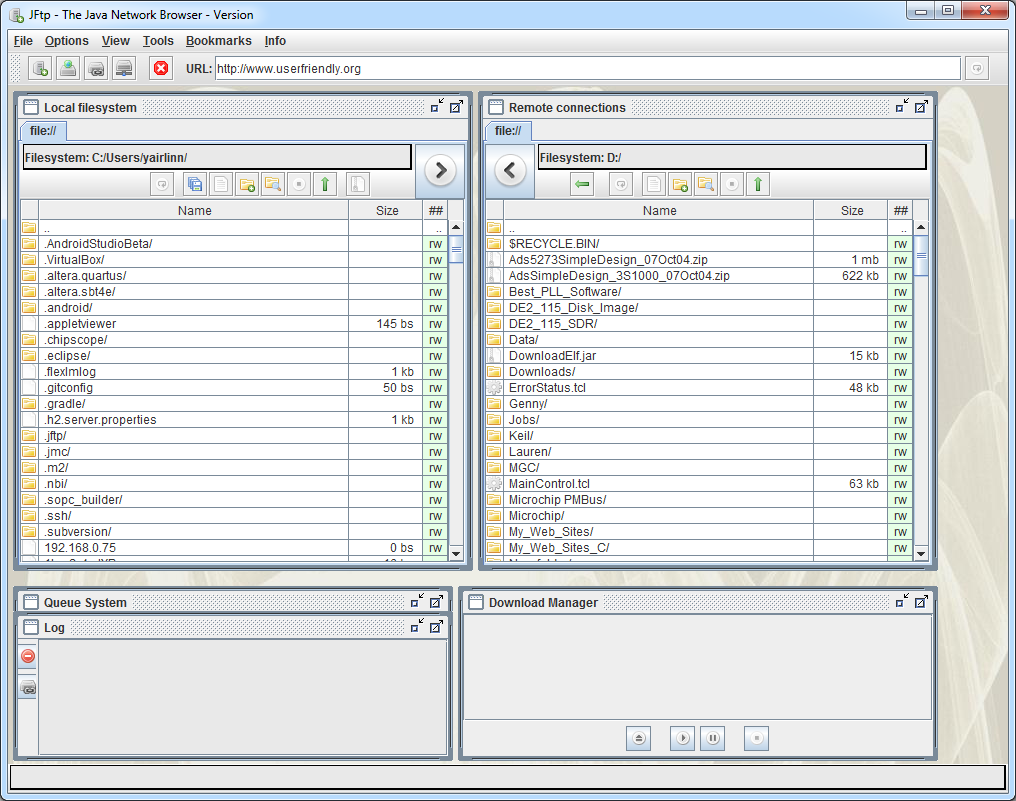
\includegraphics[width=\textwidth]{ftpTopScreen}
%\caption{General layout of the FPGA, Embedded Processors, and Memory Devices on the \gls{dtm}. Photo Credit EDEV Department (\url{https://edev.triumf.ca/projects/edevel00365/wiki/Boot_Sequence_and_Boot_Image_Selection}).}
%\label{Fig:ftpTopScreen}
%\end{figure}
%
%
%\textbf{Statix Programming}
%
%Connection to Telnet can be done via port 30 (manual command console, can be opened in Jalisco ("Open Telnet to Card") if desired) or, if desired (though not recommended) port 40 (for computer-based command interaction, which can be operated manually nonetheless). Connection should be in raw socket mode, standard telnet also seems to work well, but definitely do not use SSH.
%
%\begin{description}
%\item[Programming command:] program\_stratix\_hex\_file filename\footnote{filename is nominally stratix\_sof\_and\_elf\_image\_cropped.rbf}.
%\end{description}
%
%Programming of the flash in this method takes about 1 hour. This is due to Altera's Flash programming utilities which exhibit this performance. The time is basically limited by Altera's NIOS Flash programming board support package routines. It is unclear why those functions are four times slower than JTAG programming, and investigation is on-going as to whether this can be improved. Faster programming times will be seen if there are few changes to the binary image, in which case some unchanged blocks will not be rewritten.
%\FIXME{IS THIS STILL SLOW?}
%
%
%\textbf{Spartan Programming}
%
%Connection to Telnet can be done via port 30 (manual command console) or, if desired (though not recommended) port 40 (for computer-based command interaction, which can be operated manually nonetheless). Connection should be in raw socket mode, standard telnet also seems to work well, but definitely do not use SSH.
%
%\begin{description}
%\item[Programming command:] program\_spartan\_hex\_file filename fmc\_num
%\end{description}
%Here fmc\_num is the desired FMC so to program fmc0\_download\_raw\_bin.bin to FMC 0, the command is \textit{program\_spartan\_hex\_file fmc0\_download\_raw\_bin.bin 0}.
%
%This method allows for the programming of one \gls{fmc} at a time instead of all at once. Programming of a single FMC flash can take around 5 minutes, limited by Altera's NIOS Flash programming board support package routines. Faster programming times will be seen if there are few changes to the binary image, in which case some unchanged blocks will not be rewritten.
%
%\subsubsection{FTP Hosting}
%\subsubsection{FTP Readout}
%\begin{description}
%\item[EDEV Page:  ]\hypNote{proper readout}{https://edev.triumf.ca/projects/edevel00365/wiki/DMA_to_UDP_Transfers}
%\hypNote{manual or very low trigger rate operation}{https://edev.triumf.ca/projects/edevel00365/wiki/Software_DMA_Transactions}
%\end{description}
%

% % % % % % % % % % % % % % % % % % % % % % % % % % % % % % % % % % % %
%use this command for appendix items
\newcommand{\appItem}[4]{#1& #2& #3& \href{#4}{Link}\\ \hline}
% % % % % % % % % % % % % % % % % % % % % % % % % % % % % % % % % % % %
\chapter{Appendix}

\section{Resources $\&$ Documentation}

\subsection{Deap $\&$ TRIUMF Documents}

\begin{table}[ht]
\begin{tabular}{p{5cm} l p{7cm} l}
\textbf{Document}&	\textbf{Date}& \textbf{Description}& \textbf{Location}\\ \hline
\appItem{DEAP-3600 Electronics $\&$ DAQ Technical Design Report}{04/25/2012}{Overview of the first \gls{daq} and electronics structure, some changes have been made}{https://www.snolab.ca/deap/private/TWiki/pub/Main/TechnicalDesignReport/main.pdf}
\end{tabular}
\end{table}

\subsection{Manuals $\&$ Data Sheets}

\begin{table}[ht]
\begin{tabular}{p{5cm} l p{7cm} l}
\textbf{Document}&	\textbf{Date}& \textbf{Description}& \textbf{Location}\\
\hline
\appItem{Altera Stratix IV Overview}{}{Infomation of the Stratix IV family of FPGAs}{https://www.altera.com/products/fpga/stratix-series/stratix-iv/overview.html}
\appItem{Samtec \gls{fmc} Overview}{}{\gls{fmc} standard description}{https://www.samtec.com/standards/fmc}
\appItem{Spartan-6 Family Overview}{}{Data sheet for the Spartan-6 FPGAs used for the \gls{fmc}s}{http://www.xilinx.com/support/documentation/data_sheets/ds160.pdf}
\appItem{Altera MaxV Handbook}{}{Operations handbook for the Altera MaxV FPGA}{https://www.altera.com/content/dam/altera-www/global/en_US/pdfs/literature/hb/max-v/max5_handbook.pdf}
\appItem{ADC Data Sheet}{}{24 Channel FMC ADC}{http://www.ti.com/lit/ds/symlink/adc12eu050.pdf}
\end{tabular}
\end{table}

\subsection{Links $\&$ Websites}

\begin{table}[ht]
\begin{tabular}{p{5cm} l p{7cm} l}
\textbf{Document}&	\textbf{Date}& \textbf{Description}& \textbf{Location}\\
\hline
\appItem{Clock Distribution Module}{}{EDEV project location of the VME Clock distribution module}{https://edev.triumf.ca/project/edev/vme/edevel00163}
\appItem{\gls{fmc} HDL Submodules}{}{EDEV project location of several of the ADC board, the SFP board, and the clock cleaner HDL files}{https://edev.triumf.ca/project/firmware_software/edevel00226}
\end{tabular}
\end{table}
\chapter{Errata}
\label{chap:errata}

\section{JTAG Issues}
\subsection{USB Blaster Revision}
\begin{description}
\item[USB Blaster User Guide:]\url{https://www.altera.com/content/dam/altera-www/global/en_US/pdfs/literature/ug/ug_usb_blstr.pdf}
\end{description}
Issues have been noted using the JTAG USB blaster. It is unclear if the issue is due to the Linux software, however Rev.B of the JTAG USB Blaster wouldn't work at SNOLAB but switching to Rev.C fixed this issue. It is advised to continue using Rev.C.

\subsection{NIOS Command Shell Version}
\begin{description}
\item[USB Blaster User Guide:]\url{https://www.altera.com/content/dam/altera-www/global/en_US/pdfs/literature/ug/ug_usb_blstr.pdf}
\end{description}
When loading the firmware it is necessary to use the correct nios2\_command\_shell.sh version. For edevl00268 the Version 13.0sp1, Build 232 works reliably. However for edevel00365 (compiled with Quartus 14.1), the JTAG programming seems to be more reliable using the Quartus Version 14.1, Build 190 NIOS2 Command Shell as opposed to the 13.0sp1 with every load succeeding instead of having to flash the card a couple of times for it to work.

\NOTE{It has been previously stated that Altera Quartus Version 13.0sp1, Build 232 is used to compile hardware/software and for flash programming, while due to an Altera bug Version 12.1sp1 Build 243 is needed in order to run the system console script}

\section{VME Motherboard Version A}
Edevel00268 has never worked on the Rev.A 3xFMC motherboard and only runs on the Rev.B board even though changes between the boards are minimal. Edevel00365 however has been confirmed to work interchangeably on the revisions.

\section{Load Scripts Failing}
The flash is not always programmed correctly with the JTAG (other loading methods have yet to be throughly tested), so it is essential to check the firmware timestamp (HW Version HHDDMMYY format) on \gls{jalisco} after a flash has been preformed. Additionally to ensuring that the correct install has been made the timestamp will hint as to which of the two images is being used. With a quick glance at the hardware timestamp (see Fig. \ref{Fig:jaliscoTopScreen}) a lot of time and suffering can be averted.

%\section{VME Address}
%\label{sec:baseAddressErrata}
%changed base address
\nocite{*}
\printbibliography

\end{document}
